\documentclass{article}

\usepackage[T1]{fontenc}
\usepackage[utf8]{inputenc}
\usepackage{amsmath, amsfonts}
\usepackage{pgf}
\usepackage{subcaption}
\usepackage{graphicx}
\usepackage{lmodern}
\usepackage{microtype}
\usepackage{listings}

\author{Axel Forsman}
\title{TMA372 Assignment 1}

\begin{document}
\maketitle

\section{Question 1 and 2}\label{sec:question1}

\begin{figure}
  \begin{center}
  %% Creator: Matplotlib, PGF backend
%%
%% To include the figure in your LaTeX document, write
%%   \input{<filename>.pgf}
%%
%% Make sure the required packages are loaded in your preamble
%%   \usepackage{pgf}
%%
%% and, on pdftex
%%   \usepackage[utf8]{inputenc}\DeclareUnicodeCharacter{2212}{-}
%%
%% or, on luatex and xetex
%%   \usepackage{unicode-math}
%%
%% Figures using additional raster images can only be included by \input if
%% they are in the same directory as the main LaTeX file. For loading figures
%% from other directories you can use the `import` package
%%   \usepackage{import}
%%
%% and then include the figures with
%%   \import{<path to file>}{<filename>.pgf}
%%
%% Matplotlib used the following preamble
%%
\begingroup%
\makeatletter%
\begin{pgfpicture}%
\pgfpathrectangle{\pgfpointorigin}{\pgfqpoint{3.540000in}{3.540000in}}%
\pgfusepath{use as bounding box, clip}%
\begin{pgfscope}%
\pgfsetbuttcap%
\pgfsetmiterjoin%
\definecolor{currentfill}{rgb}{1.000000,1.000000,1.000000}%
\pgfsetfillcolor{currentfill}%
\pgfsetlinewidth{0.000000pt}%
\definecolor{currentstroke}{rgb}{1.000000,1.000000,1.000000}%
\pgfsetstrokecolor{currentstroke}%
\pgfsetdash{}{0pt}%
\pgfpathmoveto{\pgfqpoint{0.000000in}{0.000000in}}%
\pgfpathlineto{\pgfqpoint{3.540000in}{0.000000in}}%
\pgfpathlineto{\pgfqpoint{3.540000in}{3.540000in}}%
\pgfpathlineto{\pgfqpoint{0.000000in}{3.540000in}}%
\pgfpathclose%
\pgfusepath{fill}%
\end{pgfscope}%
\begin{pgfscope}%
\pgfsetbuttcap%
\pgfsetmiterjoin%
\definecolor{currentfill}{rgb}{1.000000,1.000000,1.000000}%
\pgfsetfillcolor{currentfill}%
\pgfsetlinewidth{0.000000pt}%
\definecolor{currentstroke}{rgb}{0.000000,0.000000,0.000000}%
\pgfsetstrokecolor{currentstroke}%
\pgfsetstrokeopacity{0.000000}%
\pgfsetdash{}{0pt}%
\pgfpathmoveto{\pgfqpoint{0.442500in}{0.389400in}}%
\pgfpathlineto{\pgfqpoint{3.186000in}{0.389400in}}%
\pgfpathlineto{\pgfqpoint{3.186000in}{3.115200in}}%
\pgfpathlineto{\pgfqpoint{0.442500in}{3.115200in}}%
\pgfpathclose%
\pgfusepath{fill}%
\end{pgfscope}%
\begin{pgfscope}%
\pgfsetbuttcap%
\pgfsetroundjoin%
\definecolor{currentfill}{rgb}{0.000000,0.000000,0.000000}%
\pgfsetfillcolor{currentfill}%
\pgfsetlinewidth{0.803000pt}%
\definecolor{currentstroke}{rgb}{0.000000,0.000000,0.000000}%
\pgfsetstrokecolor{currentstroke}%
\pgfsetdash{}{0pt}%
\pgfsys@defobject{currentmarker}{\pgfqpoint{0.000000in}{-0.048611in}}{\pgfqpoint{0.000000in}{0.000000in}}{%
\pgfpathmoveto{\pgfqpoint{0.000000in}{0.000000in}}%
\pgfpathlineto{\pgfqpoint{0.000000in}{-0.048611in}}%
\pgfusepath{stroke,fill}%
}%
\begin{pgfscope}%
\pgfsys@transformshift{0.567205in}{0.389400in}%
\pgfsys@useobject{currentmarker}{}%
\end{pgfscope}%
\end{pgfscope}%
\begin{pgfscope}%
\definecolor{textcolor}{rgb}{0.000000,0.000000,0.000000}%
\pgfsetstrokecolor{textcolor}%
\pgfsetfillcolor{textcolor}%
\pgftext[x=0.567205in,y=0.292178in,,top]{\color{textcolor}\rmfamily\fontsize{10.000000}{12.000000}\selectfont \(\displaystyle {0.0}\)}%
\end{pgfscope}%
\begin{pgfscope}%
\pgfsetbuttcap%
\pgfsetroundjoin%
\definecolor{currentfill}{rgb}{0.000000,0.000000,0.000000}%
\pgfsetfillcolor{currentfill}%
\pgfsetlinewidth{0.803000pt}%
\definecolor{currentstroke}{rgb}{0.000000,0.000000,0.000000}%
\pgfsetstrokecolor{currentstroke}%
\pgfsetdash{}{0pt}%
\pgfsys@defobject{currentmarker}{\pgfqpoint{0.000000in}{-0.048611in}}{\pgfqpoint{0.000000in}{0.000000in}}{%
\pgfpathmoveto{\pgfqpoint{0.000000in}{0.000000in}}%
\pgfpathlineto{\pgfqpoint{0.000000in}{-0.048611in}}%
\pgfusepath{stroke,fill}%
}%
\begin{pgfscope}%
\pgfsys@transformshift{1.066023in}{0.389400in}%
\pgfsys@useobject{currentmarker}{}%
\end{pgfscope}%
\end{pgfscope}%
\begin{pgfscope}%
\definecolor{textcolor}{rgb}{0.000000,0.000000,0.000000}%
\pgfsetstrokecolor{textcolor}%
\pgfsetfillcolor{textcolor}%
\pgftext[x=1.066023in,y=0.292178in,,top]{\color{textcolor}\rmfamily\fontsize{10.000000}{12.000000}\selectfont \(\displaystyle {0.2}\)}%
\end{pgfscope}%
\begin{pgfscope}%
\pgfsetbuttcap%
\pgfsetroundjoin%
\definecolor{currentfill}{rgb}{0.000000,0.000000,0.000000}%
\pgfsetfillcolor{currentfill}%
\pgfsetlinewidth{0.803000pt}%
\definecolor{currentstroke}{rgb}{0.000000,0.000000,0.000000}%
\pgfsetstrokecolor{currentstroke}%
\pgfsetdash{}{0pt}%
\pgfsys@defobject{currentmarker}{\pgfqpoint{0.000000in}{-0.048611in}}{\pgfqpoint{0.000000in}{0.000000in}}{%
\pgfpathmoveto{\pgfqpoint{0.000000in}{0.000000in}}%
\pgfpathlineto{\pgfqpoint{0.000000in}{-0.048611in}}%
\pgfusepath{stroke,fill}%
}%
\begin{pgfscope}%
\pgfsys@transformshift{1.564841in}{0.389400in}%
\pgfsys@useobject{currentmarker}{}%
\end{pgfscope}%
\end{pgfscope}%
\begin{pgfscope}%
\definecolor{textcolor}{rgb}{0.000000,0.000000,0.000000}%
\pgfsetstrokecolor{textcolor}%
\pgfsetfillcolor{textcolor}%
\pgftext[x=1.564841in,y=0.292178in,,top]{\color{textcolor}\rmfamily\fontsize{10.000000}{12.000000}\selectfont \(\displaystyle {0.4}\)}%
\end{pgfscope}%
\begin{pgfscope}%
\pgfsetbuttcap%
\pgfsetroundjoin%
\definecolor{currentfill}{rgb}{0.000000,0.000000,0.000000}%
\pgfsetfillcolor{currentfill}%
\pgfsetlinewidth{0.803000pt}%
\definecolor{currentstroke}{rgb}{0.000000,0.000000,0.000000}%
\pgfsetstrokecolor{currentstroke}%
\pgfsetdash{}{0pt}%
\pgfsys@defobject{currentmarker}{\pgfqpoint{0.000000in}{-0.048611in}}{\pgfqpoint{0.000000in}{0.000000in}}{%
\pgfpathmoveto{\pgfqpoint{0.000000in}{0.000000in}}%
\pgfpathlineto{\pgfqpoint{0.000000in}{-0.048611in}}%
\pgfusepath{stroke,fill}%
}%
\begin{pgfscope}%
\pgfsys@transformshift{2.063659in}{0.389400in}%
\pgfsys@useobject{currentmarker}{}%
\end{pgfscope}%
\end{pgfscope}%
\begin{pgfscope}%
\definecolor{textcolor}{rgb}{0.000000,0.000000,0.000000}%
\pgfsetstrokecolor{textcolor}%
\pgfsetfillcolor{textcolor}%
\pgftext[x=2.063659in,y=0.292178in,,top]{\color{textcolor}\rmfamily\fontsize{10.000000}{12.000000}\selectfont \(\displaystyle {0.6}\)}%
\end{pgfscope}%
\begin{pgfscope}%
\pgfsetbuttcap%
\pgfsetroundjoin%
\definecolor{currentfill}{rgb}{0.000000,0.000000,0.000000}%
\pgfsetfillcolor{currentfill}%
\pgfsetlinewidth{0.803000pt}%
\definecolor{currentstroke}{rgb}{0.000000,0.000000,0.000000}%
\pgfsetstrokecolor{currentstroke}%
\pgfsetdash{}{0pt}%
\pgfsys@defobject{currentmarker}{\pgfqpoint{0.000000in}{-0.048611in}}{\pgfqpoint{0.000000in}{0.000000in}}{%
\pgfpathmoveto{\pgfqpoint{0.000000in}{0.000000in}}%
\pgfpathlineto{\pgfqpoint{0.000000in}{-0.048611in}}%
\pgfusepath{stroke,fill}%
}%
\begin{pgfscope}%
\pgfsys@transformshift{2.562477in}{0.389400in}%
\pgfsys@useobject{currentmarker}{}%
\end{pgfscope}%
\end{pgfscope}%
\begin{pgfscope}%
\definecolor{textcolor}{rgb}{0.000000,0.000000,0.000000}%
\pgfsetstrokecolor{textcolor}%
\pgfsetfillcolor{textcolor}%
\pgftext[x=2.562477in,y=0.292178in,,top]{\color{textcolor}\rmfamily\fontsize{10.000000}{12.000000}\selectfont \(\displaystyle {0.8}\)}%
\end{pgfscope}%
\begin{pgfscope}%
\pgfsetbuttcap%
\pgfsetroundjoin%
\definecolor{currentfill}{rgb}{0.000000,0.000000,0.000000}%
\pgfsetfillcolor{currentfill}%
\pgfsetlinewidth{0.803000pt}%
\definecolor{currentstroke}{rgb}{0.000000,0.000000,0.000000}%
\pgfsetstrokecolor{currentstroke}%
\pgfsetdash{}{0pt}%
\pgfsys@defobject{currentmarker}{\pgfqpoint{0.000000in}{-0.048611in}}{\pgfqpoint{0.000000in}{0.000000in}}{%
\pgfpathmoveto{\pgfqpoint{0.000000in}{0.000000in}}%
\pgfpathlineto{\pgfqpoint{0.000000in}{-0.048611in}}%
\pgfusepath{stroke,fill}%
}%
\begin{pgfscope}%
\pgfsys@transformshift{3.061295in}{0.389400in}%
\pgfsys@useobject{currentmarker}{}%
\end{pgfscope}%
\end{pgfscope}%
\begin{pgfscope}%
\definecolor{textcolor}{rgb}{0.000000,0.000000,0.000000}%
\pgfsetstrokecolor{textcolor}%
\pgfsetfillcolor{textcolor}%
\pgftext[x=3.061295in,y=0.292178in,,top]{\color{textcolor}\rmfamily\fontsize{10.000000}{12.000000}\selectfont \(\displaystyle {1.0}\)}%
\end{pgfscope}%
\begin{pgfscope}%
\pgfsetbuttcap%
\pgfsetroundjoin%
\definecolor{currentfill}{rgb}{0.000000,0.000000,0.000000}%
\pgfsetfillcolor{currentfill}%
\pgfsetlinewidth{0.803000pt}%
\definecolor{currentstroke}{rgb}{0.000000,0.000000,0.000000}%
\pgfsetstrokecolor{currentstroke}%
\pgfsetdash{}{0pt}%
\pgfsys@defobject{currentmarker}{\pgfqpoint{-0.048611in}{0.000000in}}{\pgfqpoint{-0.000000in}{0.000000in}}{%
\pgfpathmoveto{\pgfqpoint{-0.000000in}{0.000000in}}%
\pgfpathlineto{\pgfqpoint{-0.048611in}{0.000000in}}%
\pgfusepath{stroke,fill}%
}%
\begin{pgfscope}%
\pgfsys@transformshift{0.442500in}{0.513300in}%
\pgfsys@useobject{currentmarker}{}%
\end{pgfscope}%
\end{pgfscope}%
\begin{pgfscope}%
\definecolor{textcolor}{rgb}{0.000000,0.000000,0.000000}%
\pgfsetstrokecolor{textcolor}%
\pgfsetfillcolor{textcolor}%
\pgftext[x=0.098363in, y=0.465075in, left, base]{\color{textcolor}\rmfamily\fontsize{10.000000}{12.000000}\selectfont \(\displaystyle {0.00}\)}%
\end{pgfscope}%
\begin{pgfscope}%
\pgfsetbuttcap%
\pgfsetroundjoin%
\definecolor{currentfill}{rgb}{0.000000,0.000000,0.000000}%
\pgfsetfillcolor{currentfill}%
\pgfsetlinewidth{0.803000pt}%
\definecolor{currentstroke}{rgb}{0.000000,0.000000,0.000000}%
\pgfsetstrokecolor{currentstroke}%
\pgfsetdash{}{0pt}%
\pgfsys@defobject{currentmarker}{\pgfqpoint{-0.048611in}{0.000000in}}{\pgfqpoint{-0.000000in}{0.000000in}}{%
\pgfpathmoveto{\pgfqpoint{-0.000000in}{0.000000in}}%
\pgfpathlineto{\pgfqpoint{-0.048611in}{0.000000in}}%
\pgfusepath{stroke,fill}%
}%
\begin{pgfscope}%
\pgfsys@transformshift{0.442500in}{0.830486in}%
\pgfsys@useobject{currentmarker}{}%
\end{pgfscope}%
\end{pgfscope}%
\begin{pgfscope}%
\definecolor{textcolor}{rgb}{0.000000,0.000000,0.000000}%
\pgfsetstrokecolor{textcolor}%
\pgfsetfillcolor{textcolor}%
\pgftext[x=0.098363in, y=0.782260in, left, base]{\color{textcolor}\rmfamily\fontsize{10.000000}{12.000000}\selectfont \(\displaystyle {0.05}\)}%
\end{pgfscope}%
\begin{pgfscope}%
\pgfsetbuttcap%
\pgfsetroundjoin%
\definecolor{currentfill}{rgb}{0.000000,0.000000,0.000000}%
\pgfsetfillcolor{currentfill}%
\pgfsetlinewidth{0.803000pt}%
\definecolor{currentstroke}{rgb}{0.000000,0.000000,0.000000}%
\pgfsetstrokecolor{currentstroke}%
\pgfsetdash{}{0pt}%
\pgfsys@defobject{currentmarker}{\pgfqpoint{-0.048611in}{0.000000in}}{\pgfqpoint{-0.000000in}{0.000000in}}{%
\pgfpathmoveto{\pgfqpoint{-0.000000in}{0.000000in}}%
\pgfpathlineto{\pgfqpoint{-0.048611in}{0.000000in}}%
\pgfusepath{stroke,fill}%
}%
\begin{pgfscope}%
\pgfsys@transformshift{0.442500in}{1.147672in}%
\pgfsys@useobject{currentmarker}{}%
\end{pgfscope}%
\end{pgfscope}%
\begin{pgfscope}%
\definecolor{textcolor}{rgb}{0.000000,0.000000,0.000000}%
\pgfsetstrokecolor{textcolor}%
\pgfsetfillcolor{textcolor}%
\pgftext[x=0.098363in, y=1.099446in, left, base]{\color{textcolor}\rmfamily\fontsize{10.000000}{12.000000}\selectfont \(\displaystyle {0.10}\)}%
\end{pgfscope}%
\begin{pgfscope}%
\pgfsetbuttcap%
\pgfsetroundjoin%
\definecolor{currentfill}{rgb}{0.000000,0.000000,0.000000}%
\pgfsetfillcolor{currentfill}%
\pgfsetlinewidth{0.803000pt}%
\definecolor{currentstroke}{rgb}{0.000000,0.000000,0.000000}%
\pgfsetstrokecolor{currentstroke}%
\pgfsetdash{}{0pt}%
\pgfsys@defobject{currentmarker}{\pgfqpoint{-0.048611in}{0.000000in}}{\pgfqpoint{-0.000000in}{0.000000in}}{%
\pgfpathmoveto{\pgfqpoint{-0.000000in}{0.000000in}}%
\pgfpathlineto{\pgfqpoint{-0.048611in}{0.000000in}}%
\pgfusepath{stroke,fill}%
}%
\begin{pgfscope}%
\pgfsys@transformshift{0.442500in}{1.464857in}%
\pgfsys@useobject{currentmarker}{}%
\end{pgfscope}%
\end{pgfscope}%
\begin{pgfscope}%
\definecolor{textcolor}{rgb}{0.000000,0.000000,0.000000}%
\pgfsetstrokecolor{textcolor}%
\pgfsetfillcolor{textcolor}%
\pgftext[x=0.098363in, y=1.416632in, left, base]{\color{textcolor}\rmfamily\fontsize{10.000000}{12.000000}\selectfont \(\displaystyle {0.15}\)}%
\end{pgfscope}%
\begin{pgfscope}%
\pgfsetbuttcap%
\pgfsetroundjoin%
\definecolor{currentfill}{rgb}{0.000000,0.000000,0.000000}%
\pgfsetfillcolor{currentfill}%
\pgfsetlinewidth{0.803000pt}%
\definecolor{currentstroke}{rgb}{0.000000,0.000000,0.000000}%
\pgfsetstrokecolor{currentstroke}%
\pgfsetdash{}{0pt}%
\pgfsys@defobject{currentmarker}{\pgfqpoint{-0.048611in}{0.000000in}}{\pgfqpoint{-0.000000in}{0.000000in}}{%
\pgfpathmoveto{\pgfqpoint{-0.000000in}{0.000000in}}%
\pgfpathlineto{\pgfqpoint{-0.048611in}{0.000000in}}%
\pgfusepath{stroke,fill}%
}%
\begin{pgfscope}%
\pgfsys@transformshift{0.442500in}{1.782043in}%
\pgfsys@useobject{currentmarker}{}%
\end{pgfscope}%
\end{pgfscope}%
\begin{pgfscope}%
\definecolor{textcolor}{rgb}{0.000000,0.000000,0.000000}%
\pgfsetstrokecolor{textcolor}%
\pgfsetfillcolor{textcolor}%
\pgftext[x=0.098363in, y=1.733818in, left, base]{\color{textcolor}\rmfamily\fontsize{10.000000}{12.000000}\selectfont \(\displaystyle {0.20}\)}%
\end{pgfscope}%
\begin{pgfscope}%
\pgfsetbuttcap%
\pgfsetroundjoin%
\definecolor{currentfill}{rgb}{0.000000,0.000000,0.000000}%
\pgfsetfillcolor{currentfill}%
\pgfsetlinewidth{0.803000pt}%
\definecolor{currentstroke}{rgb}{0.000000,0.000000,0.000000}%
\pgfsetstrokecolor{currentstroke}%
\pgfsetdash{}{0pt}%
\pgfsys@defobject{currentmarker}{\pgfqpoint{-0.048611in}{0.000000in}}{\pgfqpoint{-0.000000in}{0.000000in}}{%
\pgfpathmoveto{\pgfqpoint{-0.000000in}{0.000000in}}%
\pgfpathlineto{\pgfqpoint{-0.048611in}{0.000000in}}%
\pgfusepath{stroke,fill}%
}%
\begin{pgfscope}%
\pgfsys@transformshift{0.442500in}{2.099229in}%
\pgfsys@useobject{currentmarker}{}%
\end{pgfscope}%
\end{pgfscope}%
\begin{pgfscope}%
\definecolor{textcolor}{rgb}{0.000000,0.000000,0.000000}%
\pgfsetstrokecolor{textcolor}%
\pgfsetfillcolor{textcolor}%
\pgftext[x=0.098363in, y=2.051004in, left, base]{\color{textcolor}\rmfamily\fontsize{10.000000}{12.000000}\selectfont \(\displaystyle {0.25}\)}%
\end{pgfscope}%
\begin{pgfscope}%
\pgfsetbuttcap%
\pgfsetroundjoin%
\definecolor{currentfill}{rgb}{0.000000,0.000000,0.000000}%
\pgfsetfillcolor{currentfill}%
\pgfsetlinewidth{0.803000pt}%
\definecolor{currentstroke}{rgb}{0.000000,0.000000,0.000000}%
\pgfsetstrokecolor{currentstroke}%
\pgfsetdash{}{0pt}%
\pgfsys@defobject{currentmarker}{\pgfqpoint{-0.048611in}{0.000000in}}{\pgfqpoint{-0.000000in}{0.000000in}}{%
\pgfpathmoveto{\pgfqpoint{-0.000000in}{0.000000in}}%
\pgfpathlineto{\pgfqpoint{-0.048611in}{0.000000in}}%
\pgfusepath{stroke,fill}%
}%
\begin{pgfscope}%
\pgfsys@transformshift{0.442500in}{2.416415in}%
\pgfsys@useobject{currentmarker}{}%
\end{pgfscope}%
\end{pgfscope}%
\begin{pgfscope}%
\definecolor{textcolor}{rgb}{0.000000,0.000000,0.000000}%
\pgfsetstrokecolor{textcolor}%
\pgfsetfillcolor{textcolor}%
\pgftext[x=0.098363in, y=2.368189in, left, base]{\color{textcolor}\rmfamily\fontsize{10.000000}{12.000000}\selectfont \(\displaystyle {0.30}\)}%
\end{pgfscope}%
\begin{pgfscope}%
\pgfsetbuttcap%
\pgfsetroundjoin%
\definecolor{currentfill}{rgb}{0.000000,0.000000,0.000000}%
\pgfsetfillcolor{currentfill}%
\pgfsetlinewidth{0.803000pt}%
\definecolor{currentstroke}{rgb}{0.000000,0.000000,0.000000}%
\pgfsetstrokecolor{currentstroke}%
\pgfsetdash{}{0pt}%
\pgfsys@defobject{currentmarker}{\pgfqpoint{-0.048611in}{0.000000in}}{\pgfqpoint{-0.000000in}{0.000000in}}{%
\pgfpathmoveto{\pgfqpoint{-0.000000in}{0.000000in}}%
\pgfpathlineto{\pgfqpoint{-0.048611in}{0.000000in}}%
\pgfusepath{stroke,fill}%
}%
\begin{pgfscope}%
\pgfsys@transformshift{0.442500in}{2.733600in}%
\pgfsys@useobject{currentmarker}{}%
\end{pgfscope}%
\end{pgfscope}%
\begin{pgfscope}%
\definecolor{textcolor}{rgb}{0.000000,0.000000,0.000000}%
\pgfsetstrokecolor{textcolor}%
\pgfsetfillcolor{textcolor}%
\pgftext[x=0.098363in, y=2.685375in, left, base]{\color{textcolor}\rmfamily\fontsize{10.000000}{12.000000}\selectfont \(\displaystyle {0.35}\)}%
\end{pgfscope}%
\begin{pgfscope}%
\pgfsetbuttcap%
\pgfsetroundjoin%
\definecolor{currentfill}{rgb}{0.000000,0.000000,0.000000}%
\pgfsetfillcolor{currentfill}%
\pgfsetlinewidth{0.803000pt}%
\definecolor{currentstroke}{rgb}{0.000000,0.000000,0.000000}%
\pgfsetstrokecolor{currentstroke}%
\pgfsetdash{}{0pt}%
\pgfsys@defobject{currentmarker}{\pgfqpoint{-0.048611in}{0.000000in}}{\pgfqpoint{-0.000000in}{0.000000in}}{%
\pgfpathmoveto{\pgfqpoint{-0.000000in}{0.000000in}}%
\pgfpathlineto{\pgfqpoint{-0.048611in}{0.000000in}}%
\pgfusepath{stroke,fill}%
}%
\begin{pgfscope}%
\pgfsys@transformshift{0.442500in}{3.050786in}%
\pgfsys@useobject{currentmarker}{}%
\end{pgfscope}%
\end{pgfscope}%
\begin{pgfscope}%
\definecolor{textcolor}{rgb}{0.000000,0.000000,0.000000}%
\pgfsetstrokecolor{textcolor}%
\pgfsetfillcolor{textcolor}%
\pgftext[x=0.098363in, y=3.002561in, left, base]{\color{textcolor}\rmfamily\fontsize{10.000000}{12.000000}\selectfont \(\displaystyle {0.40}\)}%
\end{pgfscope}%
\begin{pgfscope}%
\pgfpathrectangle{\pgfqpoint{0.442500in}{0.389400in}}{\pgfqpoint{2.743500in}{2.725800in}}%
\pgfusepath{clip}%
\pgfsetrectcap%
\pgfsetroundjoin%
\pgfsetlinewidth{1.505625pt}%
\definecolor{currentstroke}{rgb}{0.121569,0.466667,0.705882}%
\pgfsetstrokecolor{currentstroke}%
\pgfsetdash{}{0pt}%
\pgfpathmoveto{\pgfqpoint{0.567205in}{0.513300in}}%
\pgfpathlineto{\pgfqpoint{0.753039in}{0.983345in}}%
\pgfpathlineto{\pgfqpoint{0.860627in}{1.249290in}}%
\pgfpathlineto{\pgfqpoint{0.948654in}{1.460821in}}%
\pgfpathlineto{\pgfqpoint{1.026900in}{1.642813in}}%
\pgfpathlineto{\pgfqpoint{1.095365in}{1.796432in}}%
\pgfpathlineto{\pgfqpoint{1.154049in}{1.923301in}}%
\pgfpathlineto{\pgfqpoint{1.212734in}{2.045212in}}%
\pgfpathlineto{\pgfqpoint{1.271418in}{2.161669in}}%
\pgfpathlineto{\pgfqpoint{1.320322in}{2.254192in}}%
\pgfpathlineto{\pgfqpoint{1.369226in}{2.342297in}}%
\pgfpathlineto{\pgfqpoint{1.418130in}{2.425696in}}%
\pgfpathlineto{\pgfqpoint{1.467033in}{2.504102in}}%
\pgfpathlineto{\pgfqpoint{1.506156in}{2.563039in}}%
\pgfpathlineto{\pgfqpoint{1.545279in}{2.618451in}}%
\pgfpathlineto{\pgfqpoint{1.584402in}{2.670189in}}%
\pgfpathlineto{\pgfqpoint{1.623525in}{2.718108in}}%
\pgfpathlineto{\pgfqpoint{1.662648in}{2.762061in}}%
\pgfpathlineto{\pgfqpoint{1.701771in}{2.801900in}}%
\pgfpathlineto{\pgfqpoint{1.731114in}{2.828991in}}%
\pgfpathlineto{\pgfqpoint{1.760456in}{2.853624in}}%
\pgfpathlineto{\pgfqpoint{1.789798in}{2.875736in}}%
\pgfpathlineto{\pgfqpoint{1.819140in}{2.895266in}}%
\pgfpathlineto{\pgfqpoint{1.848483in}{2.912152in}}%
\pgfpathlineto{\pgfqpoint{1.877825in}{2.926331in}}%
\pgfpathlineto{\pgfqpoint{1.907167in}{2.937742in}}%
\pgfpathlineto{\pgfqpoint{1.936509in}{2.946322in}}%
\pgfpathlineto{\pgfqpoint{1.965852in}{2.952011in}}%
\pgfpathlineto{\pgfqpoint{1.995194in}{2.954745in}}%
\pgfpathlineto{\pgfqpoint{2.024536in}{2.954462in}}%
\pgfpathlineto{\pgfqpoint{2.053878in}{2.951102in}}%
\pgfpathlineto{\pgfqpoint{2.083221in}{2.944601in}}%
\pgfpathlineto{\pgfqpoint{2.112563in}{2.934898in}}%
\pgfpathlineto{\pgfqpoint{2.141905in}{2.921931in}}%
\pgfpathlineto{\pgfqpoint{2.171247in}{2.905637in}}%
\pgfpathlineto{\pgfqpoint{2.200590in}{2.885956in}}%
\pgfpathlineto{\pgfqpoint{2.229932in}{2.862824in}}%
\pgfpathlineto{\pgfqpoint{2.259274in}{2.836180in}}%
\pgfpathlineto{\pgfqpoint{2.288616in}{2.805963in}}%
\pgfpathlineto{\pgfqpoint{2.317959in}{2.772109in}}%
\pgfpathlineto{\pgfqpoint{2.347301in}{2.734557in}}%
\pgfpathlineto{\pgfqpoint{2.376643in}{2.693245in}}%
\pgfpathlineto{\pgfqpoint{2.405985in}{2.648111in}}%
\pgfpathlineto{\pgfqpoint{2.435328in}{2.599094in}}%
\pgfpathlineto{\pgfqpoint{2.464670in}{2.546130in}}%
\pgfpathlineto{\pgfqpoint{2.494012in}{2.489158in}}%
\pgfpathlineto{\pgfqpoint{2.523354in}{2.428117in}}%
\pgfpathlineto{\pgfqpoint{2.552697in}{2.362943in}}%
\pgfpathlineto{\pgfqpoint{2.582039in}{2.293576in}}%
\pgfpathlineto{\pgfqpoint{2.621162in}{2.194456in}}%
\pgfpathlineto{\pgfqpoint{2.660285in}{2.087622in}}%
\pgfpathlineto{\pgfqpoint{2.699408in}{1.972929in}}%
\pgfpathlineto{\pgfqpoint{2.738531in}{1.850229in}}%
\pgfpathlineto{\pgfqpoint{2.777654in}{1.719376in}}%
\pgfpathlineto{\pgfqpoint{2.816777in}{1.580222in}}%
\pgfpathlineto{\pgfqpoint{2.855900in}{1.432621in}}%
\pgfpathlineto{\pgfqpoint{2.895023in}{1.276425in}}%
\pgfpathlineto{\pgfqpoint{2.934146in}{1.111489in}}%
\pgfpathlineto{\pgfqpoint{2.973269in}{0.937664in}}%
\pgfpathlineto{\pgfqpoint{3.012392in}{0.754804in}}%
\pgfpathlineto{\pgfqpoint{3.051515in}{0.562762in}}%
\pgfpathlineto{\pgfqpoint{3.061295in}{0.513300in}}%
\pgfpathlineto{\pgfqpoint{3.061295in}{0.513300in}}%
\pgfusepath{stroke}%
\end{pgfscope}%
\begin{pgfscope}%
\pgfpathrectangle{\pgfqpoint{0.442500in}{0.389400in}}{\pgfqpoint{2.743500in}{2.725800in}}%
\pgfusepath{clip}%
\pgfsetrectcap%
\pgfsetroundjoin%
\pgfsetlinewidth{1.505625pt}%
\definecolor{currentstroke}{rgb}{1.000000,0.498039,0.054902}%
\pgfsetstrokecolor{currentstroke}%
\pgfsetdash{}{0pt}%
\pgfpathmoveto{\pgfqpoint{0.567205in}{0.513300in}}%
\pgfpathlineto{\pgfqpoint{1.193172in}{2.003607in}}%
\pgfpathlineto{\pgfqpoint{1.809360in}{2.885196in}}%
\pgfpathlineto{\pgfqpoint{1.819140in}{2.889861in}}%
\pgfpathlineto{\pgfqpoint{2.435328in}{2.595998in}}%
\pgfpathlineto{\pgfqpoint{2.445108in}{2.570343in}}%
\pgfpathlineto{\pgfqpoint{3.061295in}{0.513300in}}%
\pgfpathlineto{\pgfqpoint{3.061295in}{0.513300in}}%
\pgfusepath{stroke}%
\end{pgfscope}%
\begin{pgfscope}%
\pgfpathrectangle{\pgfqpoint{0.442500in}{0.389400in}}{\pgfqpoint{2.743500in}{2.725800in}}%
\pgfusepath{clip}%
\pgfsetrectcap%
\pgfsetroundjoin%
\pgfsetlinewidth{1.505625pt}%
\definecolor{currentstroke}{rgb}{0.172549,0.627451,0.172549}%
\pgfsetstrokecolor{currentstroke}%
\pgfsetdash{}{0pt}%
\pgfpathmoveto{\pgfqpoint{0.567205in}{0.513300in}}%
\pgfpathlineto{\pgfqpoint{0.635670in}{0.705624in}}%
\pgfpathlineto{\pgfqpoint{0.704135in}{0.890777in}}%
\pgfpathlineto{\pgfqpoint{0.772600in}{1.068759in}}%
\pgfpathlineto{\pgfqpoint{0.831285in}{1.215609in}}%
\pgfpathlineto{\pgfqpoint{0.889969in}{1.357190in}}%
\pgfpathlineto{\pgfqpoint{0.948654in}{1.493503in}}%
\pgfpathlineto{\pgfqpoint{1.007338in}{1.624548in}}%
\pgfpathlineto{\pgfqpoint{1.066023in}{1.750324in}}%
\pgfpathlineto{\pgfqpoint{1.124707in}{1.870833in}}%
\pgfpathlineto{\pgfqpoint{1.183392in}{1.986074in}}%
\pgfpathlineto{\pgfqpoint{1.242076in}{2.096046in}}%
\pgfpathlineto{\pgfqpoint{1.300761in}{2.200750in}}%
\pgfpathlineto{\pgfqpoint{1.359445in}{2.300186in}}%
\pgfpathlineto{\pgfqpoint{1.408349in}{2.379025in}}%
\pgfpathlineto{\pgfqpoint{1.457253in}{2.454206in}}%
\pgfpathlineto{\pgfqpoint{1.506156in}{2.525728in}}%
\pgfpathlineto{\pgfqpoint{1.555060in}{2.593592in}}%
\pgfpathlineto{\pgfqpoint{1.603964in}{2.657798in}}%
\pgfpathlineto{\pgfqpoint{1.652868in}{2.718345in}}%
\pgfpathlineto{\pgfqpoint{1.701771in}{2.775233in}}%
\pgfpathlineto{\pgfqpoint{1.750675in}{2.828463in}}%
\pgfpathlineto{\pgfqpoint{1.799579in}{2.878035in}}%
\pgfpathlineto{\pgfqpoint{1.828921in}{2.905693in}}%
\pgfpathlineto{\pgfqpoint{1.858263in}{2.929729in}}%
\pgfpathlineto{\pgfqpoint{1.887606in}{2.949813in}}%
\pgfpathlineto{\pgfqpoint{1.907167in}{2.961008in}}%
\pgfpathlineto{\pgfqpoint{1.926729in}{2.970447in}}%
\pgfpathlineto{\pgfqpoint{1.946290in}{2.978130in}}%
\pgfpathlineto{\pgfqpoint{1.965852in}{2.984056in}}%
\pgfpathlineto{\pgfqpoint{1.985413in}{2.988227in}}%
\pgfpathlineto{\pgfqpoint{2.004975in}{2.990641in}}%
\pgfpathlineto{\pgfqpoint{2.024536in}{2.991300in}}%
\pgfpathlineto{\pgfqpoint{2.044098in}{2.990202in}}%
\pgfpathlineto{\pgfqpoint{2.063659in}{2.987349in}}%
\pgfpathlineto{\pgfqpoint{2.083221in}{2.982739in}}%
\pgfpathlineto{\pgfqpoint{2.102782in}{2.976374in}}%
\pgfpathlineto{\pgfqpoint{2.122344in}{2.968252in}}%
\pgfpathlineto{\pgfqpoint{2.141905in}{2.958374in}}%
\pgfpathlineto{\pgfqpoint{2.161467in}{2.946740in}}%
\pgfpathlineto{\pgfqpoint{2.190809in}{2.925997in}}%
\pgfpathlineto{\pgfqpoint{2.220151in}{2.901303in}}%
\pgfpathlineto{\pgfqpoint{2.249493in}{2.872657in}}%
\pgfpathlineto{\pgfqpoint{2.278836in}{2.840061in}}%
\pgfpathlineto{\pgfqpoint{2.308178in}{2.803513in}}%
\pgfpathlineto{\pgfqpoint{2.337520in}{2.763014in}}%
\pgfpathlineto{\pgfqpoint{2.366862in}{2.718564in}}%
\pgfpathlineto{\pgfqpoint{2.396205in}{2.670163in}}%
\pgfpathlineto{\pgfqpoint{2.425547in}{2.617811in}}%
\pgfpathlineto{\pgfqpoint{2.454889in}{2.561508in}}%
\pgfpathlineto{\pgfqpoint{2.484231in}{2.501253in}}%
\pgfpathlineto{\pgfqpoint{2.513574in}{2.437048in}}%
\pgfpathlineto{\pgfqpoint{2.552697in}{2.345295in}}%
\pgfpathlineto{\pgfqpoint{2.591820in}{2.246517in}}%
\pgfpathlineto{\pgfqpoint{2.630943in}{2.140715in}}%
\pgfpathlineto{\pgfqpoint{2.670066in}{2.027889in}}%
\pgfpathlineto{\pgfqpoint{2.709189in}{1.908039in}}%
\pgfpathlineto{\pgfqpoint{2.748311in}{1.781165in}}%
\pgfpathlineto{\pgfqpoint{2.787434in}{1.647267in}}%
\pgfpathlineto{\pgfqpoint{2.826557in}{1.506344in}}%
\pgfpathlineto{\pgfqpoint{2.865680in}{1.358397in}}%
\pgfpathlineto{\pgfqpoint{2.914584in}{1.163586in}}%
\pgfpathlineto{\pgfqpoint{2.963488in}{0.957799in}}%
\pgfpathlineto{\pgfqpoint{3.012392in}{0.741037in}}%
\pgfpathlineto{\pgfqpoint{3.061295in}{0.513300in}}%
\pgfpathlineto{\pgfqpoint{3.061295in}{0.513300in}}%
\pgfusepath{stroke}%
\end{pgfscope}%
\begin{pgfscope}%
\pgfsetrectcap%
\pgfsetmiterjoin%
\pgfsetlinewidth{0.803000pt}%
\definecolor{currentstroke}{rgb}{0.000000,0.000000,0.000000}%
\pgfsetstrokecolor{currentstroke}%
\pgfsetdash{}{0pt}%
\pgfpathmoveto{\pgfqpoint{0.442500in}{0.389400in}}%
\pgfpathlineto{\pgfqpoint{0.442500in}{3.115200in}}%
\pgfusepath{stroke}%
\end{pgfscope}%
\begin{pgfscope}%
\pgfsetrectcap%
\pgfsetmiterjoin%
\pgfsetlinewidth{0.803000pt}%
\definecolor{currentstroke}{rgb}{0.000000,0.000000,0.000000}%
\pgfsetstrokecolor{currentstroke}%
\pgfsetdash{}{0pt}%
\pgfpathmoveto{\pgfqpoint{3.186000in}{0.389400in}}%
\pgfpathlineto{\pgfqpoint{3.186000in}{3.115200in}}%
\pgfusepath{stroke}%
\end{pgfscope}%
\begin{pgfscope}%
\pgfsetrectcap%
\pgfsetmiterjoin%
\pgfsetlinewidth{0.803000pt}%
\definecolor{currentstroke}{rgb}{0.000000,0.000000,0.000000}%
\pgfsetstrokecolor{currentstroke}%
\pgfsetdash{}{0pt}%
\pgfpathmoveto{\pgfqpoint{0.442500in}{0.389400in}}%
\pgfpathlineto{\pgfqpoint{3.186000in}{0.389400in}}%
\pgfusepath{stroke}%
\end{pgfscope}%
\begin{pgfscope}%
\pgfsetrectcap%
\pgfsetmiterjoin%
\pgfsetlinewidth{0.803000pt}%
\definecolor{currentstroke}{rgb}{0.000000,0.000000,0.000000}%
\pgfsetstrokecolor{currentstroke}%
\pgfsetdash{}{0pt}%
\pgfpathmoveto{\pgfqpoint{0.442500in}{3.115200in}}%
\pgfpathlineto{\pgfqpoint{3.186000in}{3.115200in}}%
\pgfusepath{stroke}%
\end{pgfscope}%
\begin{pgfscope}%
\pgfsetbuttcap%
\pgfsetmiterjoin%
\definecolor{currentfill}{rgb}{1.000000,1.000000,1.000000}%
\pgfsetfillcolor{currentfill}%
\pgfsetfillopacity{0.800000}%
\pgfsetlinewidth{1.003750pt}%
\definecolor{currentstroke}{rgb}{0.800000,0.800000,0.800000}%
\pgfsetstrokecolor{currentstroke}%
\pgfsetstrokeopacity{0.800000}%
\pgfsetdash{}{0pt}%
\pgfpathmoveto{\pgfqpoint{0.539722in}{2.393749in}}%
\pgfpathlineto{\pgfqpoint{1.330731in}{2.393749in}}%
\pgfpathquadraticcurveto{\pgfqpoint{1.358508in}{2.393749in}}{\pgfqpoint{1.358508in}{2.421527in}}%
\pgfpathlineto{\pgfqpoint{1.358508in}{3.017978in}}%
\pgfpathquadraticcurveto{\pgfqpoint{1.358508in}{3.045756in}}{\pgfqpoint{1.330731in}{3.045756in}}%
\pgfpathlineto{\pgfqpoint{0.539722in}{3.045756in}}%
\pgfpathquadraticcurveto{\pgfqpoint{0.511944in}{3.045756in}}{\pgfqpoint{0.511944in}{3.017978in}}%
\pgfpathlineto{\pgfqpoint{0.511944in}{2.421527in}}%
\pgfpathquadraticcurveto{\pgfqpoint{0.511944in}{2.393749in}}{\pgfqpoint{0.539722in}{2.393749in}}%
\pgfpathclose%
\pgfusepath{stroke,fill}%
\end{pgfscope}%
\begin{pgfscope}%
\pgfsetrectcap%
\pgfsetroundjoin%
\pgfsetlinewidth{1.505625pt}%
\definecolor{currentstroke}{rgb}{0.121569,0.466667,0.705882}%
\pgfsetstrokecolor{currentstroke}%
\pgfsetdash{}{0pt}%
\pgfpathmoveto{\pgfqpoint{0.567500in}{2.941589in}}%
\pgfpathlineto{\pgfqpoint{0.845278in}{2.941589in}}%
\pgfusepath{stroke}%
\end{pgfscope}%
\begin{pgfscope}%
\definecolor{textcolor}{rgb}{0.000000,0.000000,0.000000}%
\pgfsetstrokecolor{textcolor}%
\pgfsetfillcolor{textcolor}%
\pgftext[x=0.956389in,y=2.892978in,left,base]{\color{textcolor}\rmfamily\fontsize{10.000000}{12.000000}\selectfont \(\displaystyle u\)}%
\end{pgfscope}%
\begin{pgfscope}%
\pgfsetrectcap%
\pgfsetroundjoin%
\pgfsetlinewidth{1.505625pt}%
\definecolor{currentstroke}{rgb}{1.000000,0.498039,0.054902}%
\pgfsetstrokecolor{currentstroke}%
\pgfsetdash{}{0pt}%
\pgfpathmoveto{\pgfqpoint{0.567500in}{2.740972in}}%
\pgfpathlineto{\pgfqpoint{0.845278in}{2.740972in}}%
\pgfusepath{stroke}%
\end{pgfscope}%
\begin{pgfscope}%
\definecolor{textcolor}{rgb}{0.000000,0.000000,0.000000}%
\pgfsetstrokecolor{textcolor}%
\pgfsetfillcolor{textcolor}%
\pgftext[x=0.956389in,y=2.692361in,left,base]{\color{textcolor}\rmfamily\fontsize{10.000000}{12.000000}\selectfont \(\displaystyle c\mathrm G(1)\)}%
\end{pgfscope}%
\begin{pgfscope}%
\pgfsetrectcap%
\pgfsetroundjoin%
\pgfsetlinewidth{1.505625pt}%
\definecolor{currentstroke}{rgb}{0.172549,0.627451,0.172549}%
\pgfsetstrokecolor{currentstroke}%
\pgfsetdash{}{0pt}%
\pgfpathmoveto{\pgfqpoint{0.567500in}{2.532638in}}%
\pgfpathlineto{\pgfqpoint{0.845278in}{2.532638in}}%
\pgfusepath{stroke}%
\end{pgfscope}%
\begin{pgfscope}%
\definecolor{textcolor}{rgb}{0.000000,0.000000,0.000000}%
\pgfsetstrokecolor{textcolor}%
\pgfsetfillcolor{textcolor}%
\pgftext[x=0.956389in,y=2.484027in,left,base]{\color{textcolor}\rmfamily\fontsize{10.000000}{12.000000}\selectfont \(\displaystyle c\mathrm G(2)\)}%
\end{pgfscope}%
\end{pgfpicture}%
\makeatother%
\endgroup%

  \end{center}
  \caption{The exact solution to the BVP in section~\ref{sec:question1},
    together with the $cG(1)$ and $cG(2)$ approximations
    with three inner nodes. \label{fig:1-2-cG-bvp}}
\end{figure}

Implementation is exactly as outlined in lectures.
For the $cG(2)$ approximation, in order to construct the
trial space of continuous piecewise quadratic functions on the partition of $[0,1]$,
the 2nd degree Lagrange polynomials are considered.
In order to ensure continuity they are extended,
similar to the hat functions,
while making sure that they are quadratic or zero on every subinterval of the partition.

See figure~\ref{fig:1-2-cG-bvp} for the results.
We see that the $cG(2)$ approximation is able to
match the curvature of the exact solution
a bit better than the $cG(1)$ approximation.

\section{Question 3}\label{sec:question3}

Denote the interval $[0, 1]$ by $I$.
First we find the variational formulation.
Define the space $V^0 = \{ v : I \to \mathbb R : v \in H^1(I), v(0) = v(1) = 0 \}$
of test functions.
We multiply the DE with some test function $v \in V^0$, and integrate
$$ \int_I -\epsilon u'' v + u' v \, dx = 0 $$
Using partial integration, and noting that $v$ is zero on the boundary,
we get the variational formulation
\begin{equation*}
  \text{Find $u \in V$ st. } \epsilon (u', v')_{L^2} + (u', v)_{L^2} = 0
  \quad \forall v \in V^0 \tag{VF3}
\end{equation*}
Next, for a uniform partition $T_h$ of $I$ with mesh function $h = 1 / (M + 1)$,
define the space
$V_h^0 = \{ v : I \to \mathbb R : v \text{ is cont. pw. linear on } T_h, v(0) = v(1) = 0 \}$,
$V_h = span(\varphi_0, \ldots, \varphi_m)$
The FE problem is then
\begin{equation*}\label{eq:FE3}
  \text{Find $u_h \in V_h$ st. } \epsilon (u_h', \chi')_{L^2} + (u_h', \chi)_{L^2} = 0
  \quad \forall \chi \in V_h^0 \tag{FE3}
\end{equation*}
Letting $\chi = \varphi_i$, $u_h(x) = \sum_{j=0}^M \zeta_j \varphi_j(x)$,
we note that the boundary condition $u(0) = 1$ specifies $\zeta_0 = 1$.
and inserting into \eqref{eq:FE3}, $i = 1,\ldots,M$, we get the linear system
$$ (\epsilon S + C) \chi = b $$
where $b_i = -(\epsilon (\varphi_0', \varphi_i') + (\varphi_0', \varphi_i))$.

\begin{figure}
  \begin{center}
    %% Creator: Matplotlib, PGF backend
%%
%% To include the figure in your LaTeX document, write
%%   \input{<filename>.pgf}
%%
%% Make sure the required packages are loaded in your preamble
%%   \usepackage{pgf}
%%
%% and, on pdftex
%%   \usepackage[utf8]{inputenc}\DeclareUnicodeCharacter{2212}{-}
%%
%% or, on luatex and xetex
%%   \usepackage{unicode-math}
%%
%% Figures using additional raster images can only be included by \input if
%% they are in the same directory as the main LaTeX file. For loading figures
%% from other directories you can use the `import` package
%%   \usepackage{import}
%%
%% and then include the figures with
%%   \import{<path to file>}{<filename>.pgf}
%%
%% Matplotlib used the following preamble
%%
\begingroup%
\makeatletter%
\begin{pgfpicture}%
\pgfpathrectangle{\pgfpointorigin}{\pgfqpoint{3.540000in}{3.540000in}}%
\pgfusepath{use as bounding box, clip}%
\begin{pgfscope}%
\pgfsetbuttcap%
\pgfsetmiterjoin%
\definecolor{currentfill}{rgb}{1.000000,1.000000,1.000000}%
\pgfsetfillcolor{currentfill}%
\pgfsetlinewidth{0.000000pt}%
\definecolor{currentstroke}{rgb}{1.000000,1.000000,1.000000}%
\pgfsetstrokecolor{currentstroke}%
\pgfsetdash{}{0pt}%
\pgfpathmoveto{\pgfqpoint{0.000000in}{0.000000in}}%
\pgfpathlineto{\pgfqpoint{3.540000in}{0.000000in}}%
\pgfpathlineto{\pgfqpoint{3.540000in}{3.540000in}}%
\pgfpathlineto{\pgfqpoint{0.000000in}{3.540000in}}%
\pgfpathclose%
\pgfusepath{fill}%
\end{pgfscope}%
\begin{pgfscope}%
\pgfsetbuttcap%
\pgfsetmiterjoin%
\definecolor{currentfill}{rgb}{1.000000,1.000000,1.000000}%
\pgfsetfillcolor{currentfill}%
\pgfsetlinewidth{0.000000pt}%
\definecolor{currentstroke}{rgb}{0.000000,0.000000,0.000000}%
\pgfsetstrokecolor{currentstroke}%
\pgfsetstrokeopacity{0.000000}%
\pgfsetdash{}{0pt}%
\pgfpathmoveto{\pgfqpoint{0.442500in}{0.389400in}}%
\pgfpathlineto{\pgfqpoint{3.186000in}{0.389400in}}%
\pgfpathlineto{\pgfqpoint{3.186000in}{3.115200in}}%
\pgfpathlineto{\pgfqpoint{0.442500in}{3.115200in}}%
\pgfpathclose%
\pgfusepath{fill}%
\end{pgfscope}%
\begin{pgfscope}%
\pgfsetbuttcap%
\pgfsetroundjoin%
\definecolor{currentfill}{rgb}{0.000000,0.000000,0.000000}%
\pgfsetfillcolor{currentfill}%
\pgfsetlinewidth{0.803000pt}%
\definecolor{currentstroke}{rgb}{0.000000,0.000000,0.000000}%
\pgfsetstrokecolor{currentstroke}%
\pgfsetdash{}{0pt}%
\pgfsys@defobject{currentmarker}{\pgfqpoint{0.000000in}{-0.048611in}}{\pgfqpoint{0.000000in}{0.000000in}}{%
\pgfpathmoveto{\pgfqpoint{0.000000in}{0.000000in}}%
\pgfpathlineto{\pgfqpoint{0.000000in}{-0.048611in}}%
\pgfusepath{stroke,fill}%
}%
\begin{pgfscope}%
\pgfsys@transformshift{0.567205in}{0.389400in}%
\pgfsys@useobject{currentmarker}{}%
\end{pgfscope}%
\end{pgfscope}%
\begin{pgfscope}%
\definecolor{textcolor}{rgb}{0.000000,0.000000,0.000000}%
\pgfsetstrokecolor{textcolor}%
\pgfsetfillcolor{textcolor}%
\pgftext[x=0.567205in,y=0.292178in,,top]{\color{textcolor}\rmfamily\fontsize{10.000000}{12.000000}\selectfont \(\displaystyle {0.0}\)}%
\end{pgfscope}%
\begin{pgfscope}%
\pgfsetbuttcap%
\pgfsetroundjoin%
\definecolor{currentfill}{rgb}{0.000000,0.000000,0.000000}%
\pgfsetfillcolor{currentfill}%
\pgfsetlinewidth{0.803000pt}%
\definecolor{currentstroke}{rgb}{0.000000,0.000000,0.000000}%
\pgfsetstrokecolor{currentstroke}%
\pgfsetdash{}{0pt}%
\pgfsys@defobject{currentmarker}{\pgfqpoint{0.000000in}{-0.048611in}}{\pgfqpoint{0.000000in}{0.000000in}}{%
\pgfpathmoveto{\pgfqpoint{0.000000in}{0.000000in}}%
\pgfpathlineto{\pgfqpoint{0.000000in}{-0.048611in}}%
\pgfusepath{stroke,fill}%
}%
\begin{pgfscope}%
\pgfsys@transformshift{1.066023in}{0.389400in}%
\pgfsys@useobject{currentmarker}{}%
\end{pgfscope}%
\end{pgfscope}%
\begin{pgfscope}%
\definecolor{textcolor}{rgb}{0.000000,0.000000,0.000000}%
\pgfsetstrokecolor{textcolor}%
\pgfsetfillcolor{textcolor}%
\pgftext[x=1.066023in,y=0.292178in,,top]{\color{textcolor}\rmfamily\fontsize{10.000000}{12.000000}\selectfont \(\displaystyle {0.2}\)}%
\end{pgfscope}%
\begin{pgfscope}%
\pgfsetbuttcap%
\pgfsetroundjoin%
\definecolor{currentfill}{rgb}{0.000000,0.000000,0.000000}%
\pgfsetfillcolor{currentfill}%
\pgfsetlinewidth{0.803000pt}%
\definecolor{currentstroke}{rgb}{0.000000,0.000000,0.000000}%
\pgfsetstrokecolor{currentstroke}%
\pgfsetdash{}{0pt}%
\pgfsys@defobject{currentmarker}{\pgfqpoint{0.000000in}{-0.048611in}}{\pgfqpoint{0.000000in}{0.000000in}}{%
\pgfpathmoveto{\pgfqpoint{0.000000in}{0.000000in}}%
\pgfpathlineto{\pgfqpoint{0.000000in}{-0.048611in}}%
\pgfusepath{stroke,fill}%
}%
\begin{pgfscope}%
\pgfsys@transformshift{1.564841in}{0.389400in}%
\pgfsys@useobject{currentmarker}{}%
\end{pgfscope}%
\end{pgfscope}%
\begin{pgfscope}%
\definecolor{textcolor}{rgb}{0.000000,0.000000,0.000000}%
\pgfsetstrokecolor{textcolor}%
\pgfsetfillcolor{textcolor}%
\pgftext[x=1.564841in,y=0.292178in,,top]{\color{textcolor}\rmfamily\fontsize{10.000000}{12.000000}\selectfont \(\displaystyle {0.4}\)}%
\end{pgfscope}%
\begin{pgfscope}%
\pgfsetbuttcap%
\pgfsetroundjoin%
\definecolor{currentfill}{rgb}{0.000000,0.000000,0.000000}%
\pgfsetfillcolor{currentfill}%
\pgfsetlinewidth{0.803000pt}%
\definecolor{currentstroke}{rgb}{0.000000,0.000000,0.000000}%
\pgfsetstrokecolor{currentstroke}%
\pgfsetdash{}{0pt}%
\pgfsys@defobject{currentmarker}{\pgfqpoint{0.000000in}{-0.048611in}}{\pgfqpoint{0.000000in}{0.000000in}}{%
\pgfpathmoveto{\pgfqpoint{0.000000in}{0.000000in}}%
\pgfpathlineto{\pgfqpoint{0.000000in}{-0.048611in}}%
\pgfusepath{stroke,fill}%
}%
\begin{pgfscope}%
\pgfsys@transformshift{2.063659in}{0.389400in}%
\pgfsys@useobject{currentmarker}{}%
\end{pgfscope}%
\end{pgfscope}%
\begin{pgfscope}%
\definecolor{textcolor}{rgb}{0.000000,0.000000,0.000000}%
\pgfsetstrokecolor{textcolor}%
\pgfsetfillcolor{textcolor}%
\pgftext[x=2.063659in,y=0.292178in,,top]{\color{textcolor}\rmfamily\fontsize{10.000000}{12.000000}\selectfont \(\displaystyle {0.6}\)}%
\end{pgfscope}%
\begin{pgfscope}%
\pgfsetbuttcap%
\pgfsetroundjoin%
\definecolor{currentfill}{rgb}{0.000000,0.000000,0.000000}%
\pgfsetfillcolor{currentfill}%
\pgfsetlinewidth{0.803000pt}%
\definecolor{currentstroke}{rgb}{0.000000,0.000000,0.000000}%
\pgfsetstrokecolor{currentstroke}%
\pgfsetdash{}{0pt}%
\pgfsys@defobject{currentmarker}{\pgfqpoint{0.000000in}{-0.048611in}}{\pgfqpoint{0.000000in}{0.000000in}}{%
\pgfpathmoveto{\pgfqpoint{0.000000in}{0.000000in}}%
\pgfpathlineto{\pgfqpoint{0.000000in}{-0.048611in}}%
\pgfusepath{stroke,fill}%
}%
\begin{pgfscope}%
\pgfsys@transformshift{2.562477in}{0.389400in}%
\pgfsys@useobject{currentmarker}{}%
\end{pgfscope}%
\end{pgfscope}%
\begin{pgfscope}%
\definecolor{textcolor}{rgb}{0.000000,0.000000,0.000000}%
\pgfsetstrokecolor{textcolor}%
\pgfsetfillcolor{textcolor}%
\pgftext[x=2.562477in,y=0.292178in,,top]{\color{textcolor}\rmfamily\fontsize{10.000000}{12.000000}\selectfont \(\displaystyle {0.8}\)}%
\end{pgfscope}%
\begin{pgfscope}%
\pgfsetbuttcap%
\pgfsetroundjoin%
\definecolor{currentfill}{rgb}{0.000000,0.000000,0.000000}%
\pgfsetfillcolor{currentfill}%
\pgfsetlinewidth{0.803000pt}%
\definecolor{currentstroke}{rgb}{0.000000,0.000000,0.000000}%
\pgfsetstrokecolor{currentstroke}%
\pgfsetdash{}{0pt}%
\pgfsys@defobject{currentmarker}{\pgfqpoint{0.000000in}{-0.048611in}}{\pgfqpoint{0.000000in}{0.000000in}}{%
\pgfpathmoveto{\pgfqpoint{0.000000in}{0.000000in}}%
\pgfpathlineto{\pgfqpoint{0.000000in}{-0.048611in}}%
\pgfusepath{stroke,fill}%
}%
\begin{pgfscope}%
\pgfsys@transformshift{3.061295in}{0.389400in}%
\pgfsys@useobject{currentmarker}{}%
\end{pgfscope}%
\end{pgfscope}%
\begin{pgfscope}%
\definecolor{textcolor}{rgb}{0.000000,0.000000,0.000000}%
\pgfsetstrokecolor{textcolor}%
\pgfsetfillcolor{textcolor}%
\pgftext[x=3.061295in,y=0.292178in,,top]{\color{textcolor}\rmfamily\fontsize{10.000000}{12.000000}\selectfont \(\displaystyle {1.0}\)}%
\end{pgfscope}%
\begin{pgfscope}%
\pgfsetbuttcap%
\pgfsetroundjoin%
\definecolor{currentfill}{rgb}{0.000000,0.000000,0.000000}%
\pgfsetfillcolor{currentfill}%
\pgfsetlinewidth{0.803000pt}%
\definecolor{currentstroke}{rgb}{0.000000,0.000000,0.000000}%
\pgfsetstrokecolor{currentstroke}%
\pgfsetdash{}{0pt}%
\pgfsys@defobject{currentmarker}{\pgfqpoint{-0.048611in}{0.000000in}}{\pgfqpoint{-0.000000in}{0.000000in}}{%
\pgfpathmoveto{\pgfqpoint{-0.000000in}{0.000000in}}%
\pgfpathlineto{\pgfqpoint{-0.048611in}{0.000000in}}%
\pgfusepath{stroke,fill}%
}%
\begin{pgfscope}%
\pgfsys@transformshift{0.442500in}{0.513300in}%
\pgfsys@useobject{currentmarker}{}%
\end{pgfscope}%
\end{pgfscope}%
\begin{pgfscope}%
\definecolor{textcolor}{rgb}{0.000000,0.000000,0.000000}%
\pgfsetstrokecolor{textcolor}%
\pgfsetfillcolor{textcolor}%
\pgftext[x=0.167808in, y=0.465075in, left, base]{\color{textcolor}\rmfamily\fontsize{10.000000}{12.000000}\selectfont \(\displaystyle {0.0}\)}%
\end{pgfscope}%
\begin{pgfscope}%
\pgfsetbuttcap%
\pgfsetroundjoin%
\definecolor{currentfill}{rgb}{0.000000,0.000000,0.000000}%
\pgfsetfillcolor{currentfill}%
\pgfsetlinewidth{0.803000pt}%
\definecolor{currentstroke}{rgb}{0.000000,0.000000,0.000000}%
\pgfsetstrokecolor{currentstroke}%
\pgfsetdash{}{0pt}%
\pgfsys@defobject{currentmarker}{\pgfqpoint{-0.048611in}{0.000000in}}{\pgfqpoint{-0.000000in}{0.000000in}}{%
\pgfpathmoveto{\pgfqpoint{-0.000000in}{0.000000in}}%
\pgfpathlineto{\pgfqpoint{-0.048611in}{0.000000in}}%
\pgfusepath{stroke,fill}%
}%
\begin{pgfscope}%
\pgfsys@transformshift{0.442500in}{0.820229in}%
\pgfsys@useobject{currentmarker}{}%
\end{pgfscope}%
\end{pgfscope}%
\begin{pgfscope}%
\definecolor{textcolor}{rgb}{0.000000,0.000000,0.000000}%
\pgfsetstrokecolor{textcolor}%
\pgfsetfillcolor{textcolor}%
\pgftext[x=0.167808in, y=0.772004in, left, base]{\color{textcolor}\rmfamily\fontsize{10.000000}{12.000000}\selectfont \(\displaystyle {0.2}\)}%
\end{pgfscope}%
\begin{pgfscope}%
\pgfsetbuttcap%
\pgfsetroundjoin%
\definecolor{currentfill}{rgb}{0.000000,0.000000,0.000000}%
\pgfsetfillcolor{currentfill}%
\pgfsetlinewidth{0.803000pt}%
\definecolor{currentstroke}{rgb}{0.000000,0.000000,0.000000}%
\pgfsetstrokecolor{currentstroke}%
\pgfsetdash{}{0pt}%
\pgfsys@defobject{currentmarker}{\pgfqpoint{-0.048611in}{0.000000in}}{\pgfqpoint{-0.000000in}{0.000000in}}{%
\pgfpathmoveto{\pgfqpoint{-0.000000in}{0.000000in}}%
\pgfpathlineto{\pgfqpoint{-0.048611in}{0.000000in}}%
\pgfusepath{stroke,fill}%
}%
\begin{pgfscope}%
\pgfsys@transformshift{0.442500in}{1.127158in}%
\pgfsys@useobject{currentmarker}{}%
\end{pgfscope}%
\end{pgfscope}%
\begin{pgfscope}%
\definecolor{textcolor}{rgb}{0.000000,0.000000,0.000000}%
\pgfsetstrokecolor{textcolor}%
\pgfsetfillcolor{textcolor}%
\pgftext[x=0.167808in, y=1.078933in, left, base]{\color{textcolor}\rmfamily\fontsize{10.000000}{12.000000}\selectfont \(\displaystyle {0.4}\)}%
\end{pgfscope}%
\begin{pgfscope}%
\pgfsetbuttcap%
\pgfsetroundjoin%
\definecolor{currentfill}{rgb}{0.000000,0.000000,0.000000}%
\pgfsetfillcolor{currentfill}%
\pgfsetlinewidth{0.803000pt}%
\definecolor{currentstroke}{rgb}{0.000000,0.000000,0.000000}%
\pgfsetstrokecolor{currentstroke}%
\pgfsetdash{}{0pt}%
\pgfsys@defobject{currentmarker}{\pgfqpoint{-0.048611in}{0.000000in}}{\pgfqpoint{-0.000000in}{0.000000in}}{%
\pgfpathmoveto{\pgfqpoint{-0.000000in}{0.000000in}}%
\pgfpathlineto{\pgfqpoint{-0.048611in}{0.000000in}}%
\pgfusepath{stroke,fill}%
}%
\begin{pgfscope}%
\pgfsys@transformshift{0.442500in}{1.434087in}%
\pgfsys@useobject{currentmarker}{}%
\end{pgfscope}%
\end{pgfscope}%
\begin{pgfscope}%
\definecolor{textcolor}{rgb}{0.000000,0.000000,0.000000}%
\pgfsetstrokecolor{textcolor}%
\pgfsetfillcolor{textcolor}%
\pgftext[x=0.167808in, y=1.385862in, left, base]{\color{textcolor}\rmfamily\fontsize{10.000000}{12.000000}\selectfont \(\displaystyle {0.6}\)}%
\end{pgfscope}%
\begin{pgfscope}%
\pgfsetbuttcap%
\pgfsetroundjoin%
\definecolor{currentfill}{rgb}{0.000000,0.000000,0.000000}%
\pgfsetfillcolor{currentfill}%
\pgfsetlinewidth{0.803000pt}%
\definecolor{currentstroke}{rgb}{0.000000,0.000000,0.000000}%
\pgfsetstrokecolor{currentstroke}%
\pgfsetdash{}{0pt}%
\pgfsys@defobject{currentmarker}{\pgfqpoint{-0.048611in}{0.000000in}}{\pgfqpoint{-0.000000in}{0.000000in}}{%
\pgfpathmoveto{\pgfqpoint{-0.000000in}{0.000000in}}%
\pgfpathlineto{\pgfqpoint{-0.048611in}{0.000000in}}%
\pgfusepath{stroke,fill}%
}%
\begin{pgfscope}%
\pgfsys@transformshift{0.442500in}{1.741016in}%
\pgfsys@useobject{currentmarker}{}%
\end{pgfscope}%
\end{pgfscope}%
\begin{pgfscope}%
\definecolor{textcolor}{rgb}{0.000000,0.000000,0.000000}%
\pgfsetstrokecolor{textcolor}%
\pgfsetfillcolor{textcolor}%
\pgftext[x=0.167808in, y=1.692791in, left, base]{\color{textcolor}\rmfamily\fontsize{10.000000}{12.000000}\selectfont \(\displaystyle {0.8}\)}%
\end{pgfscope}%
\begin{pgfscope}%
\pgfsetbuttcap%
\pgfsetroundjoin%
\definecolor{currentfill}{rgb}{0.000000,0.000000,0.000000}%
\pgfsetfillcolor{currentfill}%
\pgfsetlinewidth{0.803000pt}%
\definecolor{currentstroke}{rgb}{0.000000,0.000000,0.000000}%
\pgfsetstrokecolor{currentstroke}%
\pgfsetdash{}{0pt}%
\pgfsys@defobject{currentmarker}{\pgfqpoint{-0.048611in}{0.000000in}}{\pgfqpoint{-0.000000in}{0.000000in}}{%
\pgfpathmoveto{\pgfqpoint{-0.000000in}{0.000000in}}%
\pgfpathlineto{\pgfqpoint{-0.048611in}{0.000000in}}%
\pgfusepath{stroke,fill}%
}%
\begin{pgfscope}%
\pgfsys@transformshift{0.442500in}{2.047945in}%
\pgfsys@useobject{currentmarker}{}%
\end{pgfscope}%
\end{pgfscope}%
\begin{pgfscope}%
\definecolor{textcolor}{rgb}{0.000000,0.000000,0.000000}%
\pgfsetstrokecolor{textcolor}%
\pgfsetfillcolor{textcolor}%
\pgftext[x=0.167808in, y=1.999720in, left, base]{\color{textcolor}\rmfamily\fontsize{10.000000}{12.000000}\selectfont \(\displaystyle {1.0}\)}%
\end{pgfscope}%
\begin{pgfscope}%
\pgfsetbuttcap%
\pgfsetroundjoin%
\definecolor{currentfill}{rgb}{0.000000,0.000000,0.000000}%
\pgfsetfillcolor{currentfill}%
\pgfsetlinewidth{0.803000pt}%
\definecolor{currentstroke}{rgb}{0.000000,0.000000,0.000000}%
\pgfsetstrokecolor{currentstroke}%
\pgfsetdash{}{0pt}%
\pgfsys@defobject{currentmarker}{\pgfqpoint{-0.048611in}{0.000000in}}{\pgfqpoint{-0.000000in}{0.000000in}}{%
\pgfpathmoveto{\pgfqpoint{-0.000000in}{0.000000in}}%
\pgfpathlineto{\pgfqpoint{-0.048611in}{0.000000in}}%
\pgfusepath{stroke,fill}%
}%
\begin{pgfscope}%
\pgfsys@transformshift{0.442500in}{2.354874in}%
\pgfsys@useobject{currentmarker}{}%
\end{pgfscope}%
\end{pgfscope}%
\begin{pgfscope}%
\definecolor{textcolor}{rgb}{0.000000,0.000000,0.000000}%
\pgfsetstrokecolor{textcolor}%
\pgfsetfillcolor{textcolor}%
\pgftext[x=0.167808in, y=2.306649in, left, base]{\color{textcolor}\rmfamily\fontsize{10.000000}{12.000000}\selectfont \(\displaystyle {1.2}\)}%
\end{pgfscope}%
\begin{pgfscope}%
\pgfsetbuttcap%
\pgfsetroundjoin%
\definecolor{currentfill}{rgb}{0.000000,0.000000,0.000000}%
\pgfsetfillcolor{currentfill}%
\pgfsetlinewidth{0.803000pt}%
\definecolor{currentstroke}{rgb}{0.000000,0.000000,0.000000}%
\pgfsetstrokecolor{currentstroke}%
\pgfsetdash{}{0pt}%
\pgfsys@defobject{currentmarker}{\pgfqpoint{-0.048611in}{0.000000in}}{\pgfqpoint{-0.000000in}{0.000000in}}{%
\pgfpathmoveto{\pgfqpoint{-0.000000in}{0.000000in}}%
\pgfpathlineto{\pgfqpoint{-0.048611in}{0.000000in}}%
\pgfusepath{stroke,fill}%
}%
\begin{pgfscope}%
\pgfsys@transformshift{0.442500in}{2.661803in}%
\pgfsys@useobject{currentmarker}{}%
\end{pgfscope}%
\end{pgfscope}%
\begin{pgfscope}%
\definecolor{textcolor}{rgb}{0.000000,0.000000,0.000000}%
\pgfsetstrokecolor{textcolor}%
\pgfsetfillcolor{textcolor}%
\pgftext[x=0.167808in, y=2.613578in, left, base]{\color{textcolor}\rmfamily\fontsize{10.000000}{12.000000}\selectfont \(\displaystyle {1.4}\)}%
\end{pgfscope}%
\begin{pgfscope}%
\pgfsetbuttcap%
\pgfsetroundjoin%
\definecolor{currentfill}{rgb}{0.000000,0.000000,0.000000}%
\pgfsetfillcolor{currentfill}%
\pgfsetlinewidth{0.803000pt}%
\definecolor{currentstroke}{rgb}{0.000000,0.000000,0.000000}%
\pgfsetstrokecolor{currentstroke}%
\pgfsetdash{}{0pt}%
\pgfsys@defobject{currentmarker}{\pgfqpoint{-0.048611in}{0.000000in}}{\pgfqpoint{-0.000000in}{0.000000in}}{%
\pgfpathmoveto{\pgfqpoint{-0.000000in}{0.000000in}}%
\pgfpathlineto{\pgfqpoint{-0.048611in}{0.000000in}}%
\pgfusepath{stroke,fill}%
}%
\begin{pgfscope}%
\pgfsys@transformshift{0.442500in}{2.968732in}%
\pgfsys@useobject{currentmarker}{}%
\end{pgfscope}%
\end{pgfscope}%
\begin{pgfscope}%
\definecolor{textcolor}{rgb}{0.000000,0.000000,0.000000}%
\pgfsetstrokecolor{textcolor}%
\pgfsetfillcolor{textcolor}%
\pgftext[x=0.167808in, y=2.920506in, left, base]{\color{textcolor}\rmfamily\fontsize{10.000000}{12.000000}\selectfont \(\displaystyle {1.6}\)}%
\end{pgfscope}%
\begin{pgfscope}%
\pgfpathrectangle{\pgfqpoint{0.442500in}{0.389400in}}{\pgfqpoint{2.743500in}{2.725800in}}%
\pgfusepath{clip}%
\pgfsetrectcap%
\pgfsetroundjoin%
\pgfsetlinewidth{1.505625pt}%
\definecolor{currentstroke}{rgb}{0.121569,0.466667,0.705882}%
\pgfsetstrokecolor{currentstroke}%
\pgfsetdash{}{0pt}%
\pgfpathmoveto{\pgfqpoint{0.567205in}{2.047945in}}%
\pgfpathlineto{\pgfqpoint{2.875461in}{2.047053in}}%
\pgfpathlineto{\pgfqpoint{2.904803in}{2.045054in}}%
\pgfpathlineto{\pgfqpoint{2.924365in}{2.041611in}}%
\pgfpathlineto{\pgfqpoint{2.934146in}{2.038570in}}%
\pgfpathlineto{\pgfqpoint{2.943926in}{2.034069in}}%
\pgfpathlineto{\pgfqpoint{2.953707in}{2.027406in}}%
\pgfpathlineto{\pgfqpoint{2.963488in}{2.017544in}}%
\pgfpathlineto{\pgfqpoint{2.973269in}{2.002946in}}%
\pgfpathlineto{\pgfqpoint{2.983049in}{1.981339in}}%
\pgfpathlineto{\pgfqpoint{2.992830in}{1.949356in}}%
\pgfpathlineto{\pgfqpoint{3.002611in}{1.902017in}}%
\pgfpathlineto{\pgfqpoint{3.012392in}{1.831947in}}%
\pgfpathlineto{\pgfqpoint{3.022172in}{1.728231in}}%
\pgfpathlineto{\pgfqpoint{3.031953in}{1.574714in}}%
\pgfpathlineto{\pgfqpoint{3.041734in}{1.347483in}}%
\pgfpathlineto{\pgfqpoint{3.051515in}{1.011142in}}%
\pgfpathlineto{\pgfqpoint{3.061295in}{0.513300in}}%
\pgfpathlineto{\pgfqpoint{3.061295in}{0.513300in}}%
\pgfusepath{stroke}%
\end{pgfscope}%
\begin{pgfscope}%
\pgfpathrectangle{\pgfqpoint{0.442500in}{0.389400in}}{\pgfqpoint{2.743500in}{2.725800in}}%
\pgfusepath{clip}%
\pgfsetrectcap%
\pgfsetroundjoin%
\pgfsetlinewidth{1.505625pt}%
\definecolor{currentstroke}{rgb}{1.000000,0.498039,0.054902}%
\pgfsetstrokecolor{currentstroke}%
\pgfsetdash{}{0pt}%
\pgfpathmoveto{\pgfqpoint{0.567205in}{2.047945in}}%
\pgfpathlineto{\pgfqpoint{0.792162in}{2.019667in}}%
\pgfpathlineto{\pgfqpoint{0.811723in}{2.022940in}}%
\pgfpathlineto{\pgfqpoint{1.017119in}{2.063323in}}%
\pgfpathlineto{\pgfqpoint{1.026900in}{2.062109in}}%
\pgfpathlineto{\pgfqpoint{1.242076in}{1.995937in}}%
\pgfpathlineto{\pgfqpoint{1.251857in}{1.996434in}}%
\pgfpathlineto{\pgfqpoint{1.467033in}{2.099934in}}%
\pgfpathlineto{\pgfqpoint{1.476814in}{2.101349in}}%
\pgfpathlineto{\pgfqpoint{1.691991in}{1.939465in}}%
\pgfpathlineto{\pgfqpoint{1.701771in}{1.933821in}}%
\pgfpathlineto{\pgfqpoint{1.926729in}{2.198534in}}%
\pgfpathlineto{\pgfqpoint{1.936509in}{2.183215in}}%
\pgfpathlineto{\pgfqpoint{2.151686in}{1.787179in}}%
\pgfpathlineto{\pgfqpoint{2.161467in}{1.802747in}}%
\pgfpathlineto{\pgfqpoint{2.376643in}{2.422189in}}%
\pgfpathlineto{\pgfqpoint{2.386424in}{2.410965in}}%
\pgfpathlineto{\pgfqpoint{2.601600in}{1.442095in}}%
\pgfpathlineto{\pgfqpoint{2.611381in}{1.439118in}}%
\pgfpathlineto{\pgfqpoint{2.826557in}{2.954531in}}%
\pgfpathlineto{\pgfqpoint{2.836338in}{2.991300in}}%
\pgfpathlineto{\pgfqpoint{3.061295in}{0.513300in}}%
\pgfpathlineto{\pgfqpoint{3.061295in}{0.513300in}}%
\pgfusepath{stroke}%
\end{pgfscope}%
\begin{pgfscope}%
\pgfpathrectangle{\pgfqpoint{0.442500in}{0.389400in}}{\pgfqpoint{2.743500in}{2.725800in}}%
\pgfusepath{clip}%
\pgfsetrectcap%
\pgfsetroundjoin%
\pgfsetlinewidth{1.505625pt}%
\definecolor{currentstroke}{rgb}{0.172549,0.627451,0.172549}%
\pgfsetstrokecolor{currentstroke}%
\pgfsetdash{}{0pt}%
\pgfpathmoveto{\pgfqpoint{0.567205in}{2.047945in}}%
\pgfpathlineto{\pgfqpoint{0.782381in}{2.058670in}}%
\pgfpathlineto{\pgfqpoint{0.977996in}{2.041194in}}%
\pgfpathlineto{\pgfqpoint{0.987777in}{2.041470in}}%
\pgfpathlineto{\pgfqpoint{1.193172in}{2.070470in}}%
\pgfpathlineto{\pgfqpoint{1.398568in}{2.021624in}}%
\pgfpathlineto{\pgfqpoint{1.603964in}{2.101321in}}%
\pgfpathlineto{\pgfqpoint{1.613745in}{2.097626in}}%
\pgfpathlineto{\pgfqpoint{1.809360in}{1.973786in}}%
\pgfpathlineto{\pgfqpoint{1.819140in}{1.975741in}}%
\pgfpathlineto{\pgfqpoint{2.014755in}{2.177796in}}%
\pgfpathlineto{\pgfqpoint{2.024536in}{2.181252in}}%
\pgfpathlineto{\pgfqpoint{2.229932in}{1.835100in}}%
\pgfpathlineto{\pgfqpoint{2.435328in}{2.399874in}}%
\pgfpathlineto{\pgfqpoint{2.445108in}{2.373688in}}%
\pgfpathlineto{\pgfqpoint{2.640723in}{1.496095in}}%
\pgfpathlineto{\pgfqpoint{2.650504in}{1.509951in}}%
\pgfpathlineto{\pgfqpoint{2.846119in}{2.941814in}}%
\pgfpathlineto{\pgfqpoint{2.855900in}{2.966306in}}%
\pgfpathlineto{\pgfqpoint{3.061295in}{0.513300in}}%
\pgfpathlineto{\pgfqpoint{3.061295in}{0.513300in}}%
\pgfusepath{stroke}%
\end{pgfscope}%
\begin{pgfscope}%
\pgfpathrectangle{\pgfqpoint{0.442500in}{0.389400in}}{\pgfqpoint{2.743500in}{2.725800in}}%
\pgfusepath{clip}%
\pgfsetrectcap%
\pgfsetroundjoin%
\pgfsetlinewidth{1.505625pt}%
\definecolor{currentstroke}{rgb}{0.839216,0.152941,0.156863}%
\pgfsetstrokecolor{currentstroke}%
\pgfsetdash{}{0pt}%
\pgfpathmoveto{\pgfqpoint{0.567205in}{2.047945in}}%
\pgfpathlineto{\pgfqpoint{2.885242in}{2.047241in}}%
\pgfpathlineto{\pgfqpoint{2.914584in}{2.045404in}}%
\pgfpathlineto{\pgfqpoint{2.934146in}{2.041866in}}%
\pgfpathlineto{\pgfqpoint{2.943926in}{2.037933in}}%
\pgfpathlineto{\pgfqpoint{2.963488in}{2.026439in}}%
\pgfpathlineto{\pgfqpoint{2.983049in}{1.995421in}}%
\pgfpathlineto{\pgfqpoint{2.992830in}{1.962448in}}%
\pgfpathlineto{\pgfqpoint{3.012392in}{1.866151in}}%
\pgfpathlineto{\pgfqpoint{3.031953in}{1.594235in}}%
\pgfpathlineto{\pgfqpoint{3.041734in}{1.318386in}}%
\pgfpathlineto{\pgfqpoint{3.061295in}{0.513300in}}%
\pgfpathlineto{\pgfqpoint{3.061295in}{0.513300in}}%
\pgfusepath{stroke}%
\end{pgfscope}%
\begin{pgfscope}%
\pgfsetrectcap%
\pgfsetmiterjoin%
\pgfsetlinewidth{0.803000pt}%
\definecolor{currentstroke}{rgb}{0.000000,0.000000,0.000000}%
\pgfsetstrokecolor{currentstroke}%
\pgfsetdash{}{0pt}%
\pgfpathmoveto{\pgfqpoint{0.442500in}{0.389400in}}%
\pgfpathlineto{\pgfqpoint{0.442500in}{3.115200in}}%
\pgfusepath{stroke}%
\end{pgfscope}%
\begin{pgfscope}%
\pgfsetrectcap%
\pgfsetmiterjoin%
\pgfsetlinewidth{0.803000pt}%
\definecolor{currentstroke}{rgb}{0.000000,0.000000,0.000000}%
\pgfsetstrokecolor{currentstroke}%
\pgfsetdash{}{0pt}%
\pgfpathmoveto{\pgfqpoint{3.186000in}{0.389400in}}%
\pgfpathlineto{\pgfqpoint{3.186000in}{3.115200in}}%
\pgfusepath{stroke}%
\end{pgfscope}%
\begin{pgfscope}%
\pgfsetrectcap%
\pgfsetmiterjoin%
\pgfsetlinewidth{0.803000pt}%
\definecolor{currentstroke}{rgb}{0.000000,0.000000,0.000000}%
\pgfsetstrokecolor{currentstroke}%
\pgfsetdash{}{0pt}%
\pgfpathmoveto{\pgfqpoint{0.442500in}{0.389400in}}%
\pgfpathlineto{\pgfqpoint{3.186000in}{0.389400in}}%
\pgfusepath{stroke}%
\end{pgfscope}%
\begin{pgfscope}%
\pgfsetrectcap%
\pgfsetmiterjoin%
\pgfsetlinewidth{0.803000pt}%
\definecolor{currentstroke}{rgb}{0.000000,0.000000,0.000000}%
\pgfsetstrokecolor{currentstroke}%
\pgfsetdash{}{0pt}%
\pgfpathmoveto{\pgfqpoint{0.442500in}{3.115200in}}%
\pgfpathlineto{\pgfqpoint{3.186000in}{3.115200in}}%
\pgfusepath{stroke}%
\end{pgfscope}%
\begin{pgfscope}%
\pgfsetbuttcap%
\pgfsetmiterjoin%
\definecolor{currentfill}{rgb}{1.000000,1.000000,1.000000}%
\pgfsetfillcolor{currentfill}%
\pgfsetfillopacity{0.800000}%
\pgfsetlinewidth{1.003750pt}%
\definecolor{currentstroke}{rgb}{0.800000,0.800000,0.800000}%
\pgfsetstrokecolor{currentstroke}%
\pgfsetstrokeopacity{0.800000}%
\pgfsetdash{}{0pt}%
\pgfpathmoveto{\pgfqpoint{0.539722in}{0.458844in}}%
\pgfpathlineto{\pgfqpoint{1.985296in}{0.458844in}}%
\pgfpathquadraticcurveto{\pgfqpoint{2.013073in}{0.458844in}}{\pgfqpoint{2.013073in}{0.486622in}}%
\pgfpathlineto{\pgfqpoint{2.013073in}{1.291406in}}%
\pgfpathquadraticcurveto{\pgfqpoint{2.013073in}{1.319184in}}{\pgfqpoint{1.985296in}{1.319184in}}%
\pgfpathlineto{\pgfqpoint{0.539722in}{1.319184in}}%
\pgfpathquadraticcurveto{\pgfqpoint{0.511944in}{1.319184in}}{\pgfqpoint{0.511944in}{1.291406in}}%
\pgfpathlineto{\pgfqpoint{0.511944in}{0.486622in}}%
\pgfpathquadraticcurveto{\pgfqpoint{0.511944in}{0.458844in}}{\pgfqpoint{0.539722in}{0.458844in}}%
\pgfpathclose%
\pgfusepath{stroke,fill}%
\end{pgfscope}%
\begin{pgfscope}%
\pgfsetrectcap%
\pgfsetroundjoin%
\pgfsetlinewidth{1.505625pt}%
\definecolor{currentstroke}{rgb}{0.121569,0.466667,0.705882}%
\pgfsetstrokecolor{currentstroke}%
\pgfsetdash{}{0pt}%
\pgfpathmoveto{\pgfqpoint{0.567500in}{1.215017in}}%
\pgfpathlineto{\pgfqpoint{0.845278in}{1.215017in}}%
\pgfusepath{stroke}%
\end{pgfscope}%
\begin{pgfscope}%
\definecolor{textcolor}{rgb}{0.000000,0.000000,0.000000}%
\pgfsetstrokecolor{textcolor}%
\pgfsetfillcolor{textcolor}%
\pgftext[x=0.956389in,y=1.166406in,left,base]{\color{textcolor}\rmfamily\fontsize{10.000000}{12.000000}\selectfont \(\displaystyle u\)}%
\end{pgfscope}%
\begin{pgfscope}%
\pgfsetrectcap%
\pgfsetroundjoin%
\pgfsetlinewidth{1.505625pt}%
\definecolor{currentstroke}{rgb}{1.000000,0.498039,0.054902}%
\pgfsetstrokecolor{currentstroke}%
\pgfsetdash{}{0pt}%
\pgfpathmoveto{\pgfqpoint{0.567500in}{1.014400in}}%
\pgfpathlineto{\pgfqpoint{0.845278in}{1.014400in}}%
\pgfusepath{stroke}%
\end{pgfscope}%
\begin{pgfscope}%
\definecolor{textcolor}{rgb}{0.000000,0.000000,0.000000}%
\pgfsetstrokecolor{textcolor}%
\pgfsetfillcolor{textcolor}%
\pgftext[x=0.956389in,y=0.965789in,left,base]{\color{textcolor}\rmfamily\fontsize{10.000000}{12.000000}\selectfont \(\displaystyle cG(1) \quad m=10\)}%
\end{pgfscope}%
\begin{pgfscope}%
\pgfsetrectcap%
\pgfsetroundjoin%
\pgfsetlinewidth{1.505625pt}%
\definecolor{currentstroke}{rgb}{0.172549,0.627451,0.172549}%
\pgfsetstrokecolor{currentstroke}%
\pgfsetdash{}{0pt}%
\pgfpathmoveto{\pgfqpoint{0.567500in}{0.806067in}}%
\pgfpathlineto{\pgfqpoint{0.845278in}{0.806067in}}%
\pgfusepath{stroke}%
\end{pgfscope}%
\begin{pgfscope}%
\definecolor{textcolor}{rgb}{0.000000,0.000000,0.000000}%
\pgfsetstrokecolor{textcolor}%
\pgfsetfillcolor{textcolor}%
\pgftext[x=0.956389in,y=0.757456in,left,base]{\color{textcolor}\rmfamily\fontsize{10.000000}{12.000000}\selectfont \(\displaystyle cG(1) \quad m=11\)}%
\end{pgfscope}%
\begin{pgfscope}%
\pgfsetrectcap%
\pgfsetroundjoin%
\pgfsetlinewidth{1.505625pt}%
\definecolor{currentstroke}{rgb}{0.839216,0.152941,0.156863}%
\pgfsetstrokecolor{currentstroke}%
\pgfsetdash{}{0pt}%
\pgfpathmoveto{\pgfqpoint{0.567500in}{0.597733in}}%
\pgfpathlineto{\pgfqpoint{0.845278in}{0.597733in}}%
\pgfusepath{stroke}%
\end{pgfscope}%
\begin{pgfscope}%
\definecolor{textcolor}{rgb}{0.000000,0.000000,0.000000}%
\pgfsetstrokecolor{textcolor}%
\pgfsetfillcolor{textcolor}%
\pgftext[x=0.956389in,y=0.549122in,left,base]{\color{textcolor}\rmfamily\fontsize{10.000000}{12.000000}\selectfont \(\displaystyle cG(1) \quad m=100\)}%
\end{pgfscope}%
\end{pgfpicture}%
\makeatother%
\endgroup%

  \end{center}
  \caption{Results from the $cG(1)$ method for the BVP in section~\ref{sec:question3},
    for three different values of $m$, the number of inner nodes,
    together with the exact solution, $u$. \label{fig:3-cG1-bvp}}
\end{figure}

The results are given in figure~\ref{fig:3-cG1-bvp}.
There is a visible improvement when going from $m=10$ to $m=11$,
in that the peaks get smaller.
Also, we see that using $m=100$ gives a very good approximation
of the solution.

\section{Question 4}\label{sec:question4}

\subsection{4.(a)}

Start by finding the homogeneous solution $u_h$
by multiplying the DE by the integrating factor $e^{at}$
$$ \frac d {dt} \left(e^{at} u_h\right) = 0 $$
and integrating
$$ e^{at} u_h - \left. e^{at} u_h \right\vert_{t=0} = 0 $$
which gives
$$ u_h = u_h(0) e^{-at} $$
Next, for the particular solution write $u_p = C(t) e^{-at}$ and put into the DE
$$ C' e^{-at} - a C e^{at} + a C e^{-at} = t^2 $$
We see that the two terms cancel, and solve for $C$ by integrating
$$ C = \int_0^t e^{at} t^2 \, dt + \text{const} = e^{at} \left( \frac1a t^2 - \frac2{a^2} t + \frac2{a^3} \right) $$
where the second equality follows from partial integration.
Therefore
$$ u_p = C e^{-at} = \frac1a t^2 - \frac2{a^2} t + \frac2{a^3} $$
Finally, plugging in the given values of the parameters,
and finding $u_h(0)$ from the IC we get the solution
$$ u = u_h + u_p = \frac{31}{32} e^{-4t} + \left( \frac14 t^2 - \frac18 t + \frac1{32} \right) $$

\subsection{4.(b)}

For the $cG(1)$ approximation, $U$,
we consider a uniform partition of the interval $I=[0, T]$
$$ 0 = t_0 < t_1 < \cdots < t_N = T $$
and iterate from $j = 0, \ldots, N-1 $.
On every small interval $[t_j, t_{j+1}]$ we take $U$ to be
a polynomial of degree one
$$ U(t) = U_j \frac{t_{j+1} - t}{t_{j+1} - t_j} + U_{j+1} \frac{t - t_j}{t_{j+1} - t_j} $$
where $U_j$ is given by the previous iteration, $U_0 = u_0$.
Testing the DE with some $v \in \mathbb P^{(0)}(t_j, t_{j+1})$ specifies $U_{j+1}$
$$ \int_{t_j}^{t_{j+1}} (\dot U(t) + a U(t)) v(t) \, dt = \int_{t_j}^{t_{j+1}} f(t) v(t) \, dt $$
Taking $v \equiv 1$ to be the basis function and solving for $U_{j+1}$ we get
$$ U_{j+1} = \frac{U_j \left( 1 + \frac12 a h \right) + \int_{t_j}^{t_{j+1}} f(t) \, dt}{1 - \frac12 a h} $$
where $h = t_{j+1} - t_j$.

\begin{figure}
  \begin{center}
  %% Creator: Matplotlib, PGF backend
%%
%% To include the figure in your LaTeX document, write
%%   \input{<filename>.pgf}
%%
%% Make sure the required packages are loaded in your preamble
%%   \usepackage{pgf}
%%
%% and, on pdftex
%%   \usepackage[utf8]{inputenc}\DeclareUnicodeCharacter{2212}{-}
%%
%% or, on luatex and xetex
%%   \usepackage{unicode-math}
%%
%% Figures using additional raster images can only be included by \input if
%% they are in the same directory as the main LaTeX file. For loading figures
%% from other directories you can use the `import` package
%%   \usepackage{import}
%%
%% and then include the figures with
%%   \import{<path to file>}{<filename>.pgf}
%%
%% Matplotlib used the following preamble
%%
\begingroup%
\makeatletter%
\begin{pgfpicture}%
\pgfpathrectangle{\pgfpointorigin}{\pgfqpoint{3.540000in}{3.540000in}}%
\pgfusepath{use as bounding box, clip}%
\begin{pgfscope}%
\pgfsetbuttcap%
\pgfsetmiterjoin%
\definecolor{currentfill}{rgb}{1.000000,1.000000,1.000000}%
\pgfsetfillcolor{currentfill}%
\pgfsetlinewidth{0.000000pt}%
\definecolor{currentstroke}{rgb}{1.000000,1.000000,1.000000}%
\pgfsetstrokecolor{currentstroke}%
\pgfsetdash{}{0pt}%
\pgfpathmoveto{\pgfqpoint{0.000000in}{0.000000in}}%
\pgfpathlineto{\pgfqpoint{3.540000in}{0.000000in}}%
\pgfpathlineto{\pgfqpoint{3.540000in}{3.540000in}}%
\pgfpathlineto{\pgfqpoint{0.000000in}{3.540000in}}%
\pgfpathclose%
\pgfusepath{fill}%
\end{pgfscope}%
\begin{pgfscope}%
\pgfsetbuttcap%
\pgfsetmiterjoin%
\definecolor{currentfill}{rgb}{1.000000,1.000000,1.000000}%
\pgfsetfillcolor{currentfill}%
\pgfsetlinewidth{0.000000pt}%
\definecolor{currentstroke}{rgb}{0.000000,0.000000,0.000000}%
\pgfsetstrokecolor{currentstroke}%
\pgfsetstrokeopacity{0.000000}%
\pgfsetdash{}{0pt}%
\pgfpathmoveto{\pgfqpoint{0.442500in}{0.389400in}}%
\pgfpathlineto{\pgfqpoint{3.186000in}{0.389400in}}%
\pgfpathlineto{\pgfqpoint{3.186000in}{3.115200in}}%
\pgfpathlineto{\pgfqpoint{0.442500in}{3.115200in}}%
\pgfpathclose%
\pgfusepath{fill}%
\end{pgfscope}%
\begin{pgfscope}%
\pgfsetbuttcap%
\pgfsetroundjoin%
\definecolor{currentfill}{rgb}{0.000000,0.000000,0.000000}%
\pgfsetfillcolor{currentfill}%
\pgfsetlinewidth{0.803000pt}%
\definecolor{currentstroke}{rgb}{0.000000,0.000000,0.000000}%
\pgfsetstrokecolor{currentstroke}%
\pgfsetdash{}{0pt}%
\pgfsys@defobject{currentmarker}{\pgfqpoint{0.000000in}{-0.048611in}}{\pgfqpoint{0.000000in}{0.000000in}}{%
\pgfpathmoveto{\pgfqpoint{0.000000in}{0.000000in}}%
\pgfpathlineto{\pgfqpoint{0.000000in}{-0.048611in}}%
\pgfusepath{stroke,fill}%
}%
\begin{pgfscope}%
\pgfsys@transformshift{0.567205in}{0.389400in}%
\pgfsys@useobject{currentmarker}{}%
\end{pgfscope}%
\end{pgfscope}%
\begin{pgfscope}%
\definecolor{textcolor}{rgb}{0.000000,0.000000,0.000000}%
\pgfsetstrokecolor{textcolor}%
\pgfsetfillcolor{textcolor}%
\pgftext[x=0.567205in,y=0.292178in,,top]{\color{textcolor}\rmfamily\fontsize{10.000000}{12.000000}\selectfont \(\displaystyle {0.0}\)}%
\end{pgfscope}%
\begin{pgfscope}%
\pgfsetbuttcap%
\pgfsetroundjoin%
\definecolor{currentfill}{rgb}{0.000000,0.000000,0.000000}%
\pgfsetfillcolor{currentfill}%
\pgfsetlinewidth{0.803000pt}%
\definecolor{currentstroke}{rgb}{0.000000,0.000000,0.000000}%
\pgfsetstrokecolor{currentstroke}%
\pgfsetdash{}{0pt}%
\pgfsys@defobject{currentmarker}{\pgfqpoint{0.000000in}{-0.048611in}}{\pgfqpoint{0.000000in}{0.000000in}}{%
\pgfpathmoveto{\pgfqpoint{0.000000in}{0.000000in}}%
\pgfpathlineto{\pgfqpoint{0.000000in}{-0.048611in}}%
\pgfusepath{stroke,fill}%
}%
\begin{pgfscope}%
\pgfsys@transformshift{1.066023in}{0.389400in}%
\pgfsys@useobject{currentmarker}{}%
\end{pgfscope}%
\end{pgfscope}%
\begin{pgfscope}%
\definecolor{textcolor}{rgb}{0.000000,0.000000,0.000000}%
\pgfsetstrokecolor{textcolor}%
\pgfsetfillcolor{textcolor}%
\pgftext[x=1.066023in,y=0.292178in,,top]{\color{textcolor}\rmfamily\fontsize{10.000000}{12.000000}\selectfont \(\displaystyle {0.2}\)}%
\end{pgfscope}%
\begin{pgfscope}%
\pgfsetbuttcap%
\pgfsetroundjoin%
\definecolor{currentfill}{rgb}{0.000000,0.000000,0.000000}%
\pgfsetfillcolor{currentfill}%
\pgfsetlinewidth{0.803000pt}%
\definecolor{currentstroke}{rgb}{0.000000,0.000000,0.000000}%
\pgfsetstrokecolor{currentstroke}%
\pgfsetdash{}{0pt}%
\pgfsys@defobject{currentmarker}{\pgfqpoint{0.000000in}{-0.048611in}}{\pgfqpoint{0.000000in}{0.000000in}}{%
\pgfpathmoveto{\pgfqpoint{0.000000in}{0.000000in}}%
\pgfpathlineto{\pgfqpoint{0.000000in}{-0.048611in}}%
\pgfusepath{stroke,fill}%
}%
\begin{pgfscope}%
\pgfsys@transformshift{1.564841in}{0.389400in}%
\pgfsys@useobject{currentmarker}{}%
\end{pgfscope}%
\end{pgfscope}%
\begin{pgfscope}%
\definecolor{textcolor}{rgb}{0.000000,0.000000,0.000000}%
\pgfsetstrokecolor{textcolor}%
\pgfsetfillcolor{textcolor}%
\pgftext[x=1.564841in,y=0.292178in,,top]{\color{textcolor}\rmfamily\fontsize{10.000000}{12.000000}\selectfont \(\displaystyle {0.4}\)}%
\end{pgfscope}%
\begin{pgfscope}%
\pgfsetbuttcap%
\pgfsetroundjoin%
\definecolor{currentfill}{rgb}{0.000000,0.000000,0.000000}%
\pgfsetfillcolor{currentfill}%
\pgfsetlinewidth{0.803000pt}%
\definecolor{currentstroke}{rgb}{0.000000,0.000000,0.000000}%
\pgfsetstrokecolor{currentstroke}%
\pgfsetdash{}{0pt}%
\pgfsys@defobject{currentmarker}{\pgfqpoint{0.000000in}{-0.048611in}}{\pgfqpoint{0.000000in}{0.000000in}}{%
\pgfpathmoveto{\pgfqpoint{0.000000in}{0.000000in}}%
\pgfpathlineto{\pgfqpoint{0.000000in}{-0.048611in}}%
\pgfusepath{stroke,fill}%
}%
\begin{pgfscope}%
\pgfsys@transformshift{2.063659in}{0.389400in}%
\pgfsys@useobject{currentmarker}{}%
\end{pgfscope}%
\end{pgfscope}%
\begin{pgfscope}%
\definecolor{textcolor}{rgb}{0.000000,0.000000,0.000000}%
\pgfsetstrokecolor{textcolor}%
\pgfsetfillcolor{textcolor}%
\pgftext[x=2.063659in,y=0.292178in,,top]{\color{textcolor}\rmfamily\fontsize{10.000000}{12.000000}\selectfont \(\displaystyle {0.6}\)}%
\end{pgfscope}%
\begin{pgfscope}%
\pgfsetbuttcap%
\pgfsetroundjoin%
\definecolor{currentfill}{rgb}{0.000000,0.000000,0.000000}%
\pgfsetfillcolor{currentfill}%
\pgfsetlinewidth{0.803000pt}%
\definecolor{currentstroke}{rgb}{0.000000,0.000000,0.000000}%
\pgfsetstrokecolor{currentstroke}%
\pgfsetdash{}{0pt}%
\pgfsys@defobject{currentmarker}{\pgfqpoint{0.000000in}{-0.048611in}}{\pgfqpoint{0.000000in}{0.000000in}}{%
\pgfpathmoveto{\pgfqpoint{0.000000in}{0.000000in}}%
\pgfpathlineto{\pgfqpoint{0.000000in}{-0.048611in}}%
\pgfusepath{stroke,fill}%
}%
\begin{pgfscope}%
\pgfsys@transformshift{2.562477in}{0.389400in}%
\pgfsys@useobject{currentmarker}{}%
\end{pgfscope}%
\end{pgfscope}%
\begin{pgfscope}%
\definecolor{textcolor}{rgb}{0.000000,0.000000,0.000000}%
\pgfsetstrokecolor{textcolor}%
\pgfsetfillcolor{textcolor}%
\pgftext[x=2.562477in,y=0.292178in,,top]{\color{textcolor}\rmfamily\fontsize{10.000000}{12.000000}\selectfont \(\displaystyle {0.8}\)}%
\end{pgfscope}%
\begin{pgfscope}%
\pgfsetbuttcap%
\pgfsetroundjoin%
\definecolor{currentfill}{rgb}{0.000000,0.000000,0.000000}%
\pgfsetfillcolor{currentfill}%
\pgfsetlinewidth{0.803000pt}%
\definecolor{currentstroke}{rgb}{0.000000,0.000000,0.000000}%
\pgfsetstrokecolor{currentstroke}%
\pgfsetdash{}{0pt}%
\pgfsys@defobject{currentmarker}{\pgfqpoint{0.000000in}{-0.048611in}}{\pgfqpoint{0.000000in}{0.000000in}}{%
\pgfpathmoveto{\pgfqpoint{0.000000in}{0.000000in}}%
\pgfpathlineto{\pgfqpoint{0.000000in}{-0.048611in}}%
\pgfusepath{stroke,fill}%
}%
\begin{pgfscope}%
\pgfsys@transformshift{3.061295in}{0.389400in}%
\pgfsys@useobject{currentmarker}{}%
\end{pgfscope}%
\end{pgfscope}%
\begin{pgfscope}%
\definecolor{textcolor}{rgb}{0.000000,0.000000,0.000000}%
\pgfsetstrokecolor{textcolor}%
\pgfsetfillcolor{textcolor}%
\pgftext[x=3.061295in,y=0.292178in,,top]{\color{textcolor}\rmfamily\fontsize{10.000000}{12.000000}\selectfont \(\displaystyle {1.0}\)}%
\end{pgfscope}%
\begin{pgfscope}%
\pgfsetbuttcap%
\pgfsetroundjoin%
\definecolor{currentfill}{rgb}{0.000000,0.000000,0.000000}%
\pgfsetfillcolor{currentfill}%
\pgfsetlinewidth{0.803000pt}%
\definecolor{currentstroke}{rgb}{0.000000,0.000000,0.000000}%
\pgfsetstrokecolor{currentstroke}%
\pgfsetdash{}{0pt}%
\pgfsys@defobject{currentmarker}{\pgfqpoint{-0.048611in}{0.000000in}}{\pgfqpoint{-0.000000in}{0.000000in}}{%
\pgfpathmoveto{\pgfqpoint{-0.000000in}{0.000000in}}%
\pgfpathlineto{\pgfqpoint{-0.048611in}{0.000000in}}%
\pgfusepath{stroke,fill}%
}%
\begin{pgfscope}%
\pgfsys@transformshift{0.442500in}{0.759885in}%
\pgfsys@useobject{currentmarker}{}%
\end{pgfscope}%
\end{pgfscope}%
\begin{pgfscope}%
\definecolor{textcolor}{rgb}{0.000000,0.000000,0.000000}%
\pgfsetstrokecolor{textcolor}%
\pgfsetfillcolor{textcolor}%
\pgftext[x=0.167808in, y=0.711659in, left, base]{\color{textcolor}\rmfamily\fontsize{10.000000}{12.000000}\selectfont \(\displaystyle {0.2}\)}%
\end{pgfscope}%
\begin{pgfscope}%
\pgfsetbuttcap%
\pgfsetroundjoin%
\definecolor{currentfill}{rgb}{0.000000,0.000000,0.000000}%
\pgfsetfillcolor{currentfill}%
\pgfsetlinewidth{0.803000pt}%
\definecolor{currentstroke}{rgb}{0.000000,0.000000,0.000000}%
\pgfsetstrokecolor{currentstroke}%
\pgfsetdash{}{0pt}%
\pgfsys@defobject{currentmarker}{\pgfqpoint{-0.048611in}{0.000000in}}{\pgfqpoint{-0.000000in}{0.000000in}}{%
\pgfpathmoveto{\pgfqpoint{-0.000000in}{0.000000in}}%
\pgfpathlineto{\pgfqpoint{-0.048611in}{0.000000in}}%
\pgfusepath{stroke,fill}%
}%
\begin{pgfscope}%
\pgfsys@transformshift{0.442500in}{1.317738in}%
\pgfsys@useobject{currentmarker}{}%
\end{pgfscope}%
\end{pgfscope}%
\begin{pgfscope}%
\definecolor{textcolor}{rgb}{0.000000,0.000000,0.000000}%
\pgfsetstrokecolor{textcolor}%
\pgfsetfillcolor{textcolor}%
\pgftext[x=0.167808in, y=1.269513in, left, base]{\color{textcolor}\rmfamily\fontsize{10.000000}{12.000000}\selectfont \(\displaystyle {0.4}\)}%
\end{pgfscope}%
\begin{pgfscope}%
\pgfsetbuttcap%
\pgfsetroundjoin%
\definecolor{currentfill}{rgb}{0.000000,0.000000,0.000000}%
\pgfsetfillcolor{currentfill}%
\pgfsetlinewidth{0.803000pt}%
\definecolor{currentstroke}{rgb}{0.000000,0.000000,0.000000}%
\pgfsetstrokecolor{currentstroke}%
\pgfsetdash{}{0pt}%
\pgfsys@defobject{currentmarker}{\pgfqpoint{-0.048611in}{0.000000in}}{\pgfqpoint{-0.000000in}{0.000000in}}{%
\pgfpathmoveto{\pgfqpoint{-0.000000in}{0.000000in}}%
\pgfpathlineto{\pgfqpoint{-0.048611in}{0.000000in}}%
\pgfusepath{stroke,fill}%
}%
\begin{pgfscope}%
\pgfsys@transformshift{0.442500in}{1.875592in}%
\pgfsys@useobject{currentmarker}{}%
\end{pgfscope}%
\end{pgfscope}%
\begin{pgfscope}%
\definecolor{textcolor}{rgb}{0.000000,0.000000,0.000000}%
\pgfsetstrokecolor{textcolor}%
\pgfsetfillcolor{textcolor}%
\pgftext[x=0.167808in, y=1.827367in, left, base]{\color{textcolor}\rmfamily\fontsize{10.000000}{12.000000}\selectfont \(\displaystyle {0.6}\)}%
\end{pgfscope}%
\begin{pgfscope}%
\pgfsetbuttcap%
\pgfsetroundjoin%
\definecolor{currentfill}{rgb}{0.000000,0.000000,0.000000}%
\pgfsetfillcolor{currentfill}%
\pgfsetlinewidth{0.803000pt}%
\definecolor{currentstroke}{rgb}{0.000000,0.000000,0.000000}%
\pgfsetstrokecolor{currentstroke}%
\pgfsetdash{}{0pt}%
\pgfsys@defobject{currentmarker}{\pgfqpoint{-0.048611in}{0.000000in}}{\pgfqpoint{-0.000000in}{0.000000in}}{%
\pgfpathmoveto{\pgfqpoint{-0.000000in}{0.000000in}}%
\pgfpathlineto{\pgfqpoint{-0.048611in}{0.000000in}}%
\pgfusepath{stroke,fill}%
}%
\begin{pgfscope}%
\pgfsys@transformshift{0.442500in}{2.433446in}%
\pgfsys@useobject{currentmarker}{}%
\end{pgfscope}%
\end{pgfscope}%
\begin{pgfscope}%
\definecolor{textcolor}{rgb}{0.000000,0.000000,0.000000}%
\pgfsetstrokecolor{textcolor}%
\pgfsetfillcolor{textcolor}%
\pgftext[x=0.167808in, y=2.385221in, left, base]{\color{textcolor}\rmfamily\fontsize{10.000000}{12.000000}\selectfont \(\displaystyle {0.8}\)}%
\end{pgfscope}%
\begin{pgfscope}%
\pgfsetbuttcap%
\pgfsetroundjoin%
\definecolor{currentfill}{rgb}{0.000000,0.000000,0.000000}%
\pgfsetfillcolor{currentfill}%
\pgfsetlinewidth{0.803000pt}%
\definecolor{currentstroke}{rgb}{0.000000,0.000000,0.000000}%
\pgfsetstrokecolor{currentstroke}%
\pgfsetdash{}{0pt}%
\pgfsys@defobject{currentmarker}{\pgfqpoint{-0.048611in}{0.000000in}}{\pgfqpoint{-0.000000in}{0.000000in}}{%
\pgfpathmoveto{\pgfqpoint{-0.000000in}{0.000000in}}%
\pgfpathlineto{\pgfqpoint{-0.048611in}{0.000000in}}%
\pgfusepath{stroke,fill}%
}%
\begin{pgfscope}%
\pgfsys@transformshift{0.442500in}{2.991300in}%
\pgfsys@useobject{currentmarker}{}%
\end{pgfscope}%
\end{pgfscope}%
\begin{pgfscope}%
\definecolor{textcolor}{rgb}{0.000000,0.000000,0.000000}%
\pgfsetstrokecolor{textcolor}%
\pgfsetfillcolor{textcolor}%
\pgftext[x=0.167808in, y=2.943075in, left, base]{\color{textcolor}\rmfamily\fontsize{10.000000}{12.000000}\selectfont \(\displaystyle {1.0}\)}%
\end{pgfscope}%
\begin{pgfscope}%
\pgfpathrectangle{\pgfqpoint{0.442500in}{0.389400in}}{\pgfqpoint{2.743500in}{2.725800in}}%
\pgfusepath{clip}%
\pgfsetrectcap%
\pgfsetroundjoin%
\pgfsetlinewidth{1.505625pt}%
\definecolor{currentstroke}{rgb}{0.121569,0.466667,0.705882}%
\pgfsetstrokecolor{currentstroke}%
\pgfsetdash{}{0pt}%
\pgfpathmoveto{\pgfqpoint{0.567205in}{2.991300in}}%
\pgfpathlineto{\pgfqpoint{0.606328in}{2.821668in}}%
\pgfpathlineto{\pgfqpoint{0.645451in}{2.662374in}}%
\pgfpathlineto{\pgfqpoint{0.684574in}{2.512809in}}%
\pgfpathlineto{\pgfqpoint{0.723697in}{2.372403in}}%
\pgfpathlineto{\pgfqpoint{0.762820in}{2.240620in}}%
\pgfpathlineto{\pgfqpoint{0.801943in}{2.116956in}}%
\pgfpathlineto{\pgfqpoint{0.841066in}{2.000938in}}%
\pgfpathlineto{\pgfqpoint{0.880189in}{1.892122in}}%
\pgfpathlineto{\pgfqpoint{0.919311in}{1.790091in}}%
\pgfpathlineto{\pgfqpoint{0.958434in}{1.694454in}}%
\pgfpathlineto{\pgfqpoint{0.997557in}{1.604841in}}%
\pgfpathlineto{\pgfqpoint{1.036680in}{1.520909in}}%
\pgfpathlineto{\pgfqpoint{1.075803in}{1.442331in}}%
\pgfpathlineto{\pgfqpoint{1.114926in}{1.368803in}}%
\pgfpathlineto{\pgfqpoint{1.154049in}{1.300040in}}%
\pgfpathlineto{\pgfqpoint{1.193172in}{1.235772in}}%
\pgfpathlineto{\pgfqpoint{1.232295in}{1.175746in}}%
\pgfpathlineto{\pgfqpoint{1.271418in}{1.119726in}}%
\pgfpathlineto{\pgfqpoint{1.310541in}{1.067489in}}%
\pgfpathlineto{\pgfqpoint{1.349664in}{1.018825in}}%
\pgfpathlineto{\pgfqpoint{1.388787in}{0.973538in}}%
\pgfpathlineto{\pgfqpoint{1.427910in}{0.931444in}}%
\pgfpathlineto{\pgfqpoint{1.467033in}{0.892370in}}%
\pgfpathlineto{\pgfqpoint{1.506156in}{0.856151in}}%
\pgfpathlineto{\pgfqpoint{1.545279in}{0.822637in}}%
\pgfpathlineto{\pgfqpoint{1.584402in}{0.791682in}}%
\pgfpathlineto{\pgfqpoint{1.623525in}{0.763153in}}%
\pgfpathlineto{\pgfqpoint{1.662648in}{0.736923in}}%
\pgfpathlineto{\pgfqpoint{1.701771in}{0.712872in}}%
\pgfpathlineto{\pgfqpoint{1.750675in}{0.685704in}}%
\pgfpathlineto{\pgfqpoint{1.799579in}{0.661565in}}%
\pgfpathlineto{\pgfqpoint{1.848483in}{0.640266in}}%
\pgfpathlineto{\pgfqpoint{1.897386in}{0.621634in}}%
\pgfpathlineto{\pgfqpoint{1.946290in}{0.605508in}}%
\pgfpathlineto{\pgfqpoint{1.995194in}{0.591739in}}%
\pgfpathlineto{\pgfqpoint{2.044098in}{0.580191in}}%
\pgfpathlineto{\pgfqpoint{2.093001in}{0.570735in}}%
\pgfpathlineto{\pgfqpoint{2.141905in}{0.563254in}}%
\pgfpathlineto{\pgfqpoint{2.200590in}{0.556733in}}%
\pgfpathlineto{\pgfqpoint{2.259274in}{0.552729in}}%
\pgfpathlineto{\pgfqpoint{2.317959in}{0.551085in}}%
\pgfpathlineto{\pgfqpoint{2.376643in}{0.551657in}}%
\pgfpathlineto{\pgfqpoint{2.435328in}{0.554318in}}%
\pgfpathlineto{\pgfqpoint{2.494012in}{0.558948in}}%
\pgfpathlineto{\pgfqpoint{2.562477in}{0.566695in}}%
\pgfpathlineto{\pgfqpoint{2.630943in}{0.576823in}}%
\pgfpathlineto{\pgfqpoint{2.699408in}{0.589193in}}%
\pgfpathlineto{\pgfqpoint{2.767873in}{0.603681in}}%
\pgfpathlineto{\pgfqpoint{2.846119in}{0.622691in}}%
\pgfpathlineto{\pgfqpoint{2.924365in}{0.644175in}}%
\pgfpathlineto{\pgfqpoint{3.002611in}{0.668004in}}%
\pgfpathlineto{\pgfqpoint{3.061295in}{0.687345in}}%
\pgfpathlineto{\pgfqpoint{3.061295in}{0.687345in}}%
\pgfusepath{stroke}%
\end{pgfscope}%
\begin{pgfscope}%
\pgfpathrectangle{\pgfqpoint{0.442500in}{0.389400in}}{\pgfqpoint{2.743500in}{2.725800in}}%
\pgfusepath{clip}%
\pgfsetrectcap%
\pgfsetroundjoin%
\pgfsetlinewidth{1.505625pt}%
\definecolor{currentstroke}{rgb}{1.000000,0.498039,0.054902}%
\pgfsetstrokecolor{currentstroke}%
\pgfsetdash{}{0pt}%
\pgfpathmoveto{\pgfqpoint{0.567205in}{2.991300in}}%
\pgfpathlineto{\pgfqpoint{1.183392in}{1.163235in}}%
\pgfpathlineto{\pgfqpoint{1.193172in}{1.139282in}}%
\pgfpathlineto{\pgfqpoint{1.809360in}{0.587353in}}%
\pgfpathlineto{\pgfqpoint{1.819140in}{0.582424in}}%
\pgfpathlineto{\pgfqpoint{2.435328in}{0.513300in}}%
\pgfpathlineto{\pgfqpoint{2.454889in}{0.517171in}}%
\pgfpathlineto{\pgfqpoint{3.061295in}{0.664039in}}%
\pgfpathlineto{\pgfqpoint{3.061295in}{0.664039in}}%
\pgfusepath{stroke}%
\end{pgfscope}%
\begin{pgfscope}%
\pgfpathrectangle{\pgfqpoint{0.442500in}{0.389400in}}{\pgfqpoint{2.743500in}{2.725800in}}%
\pgfusepath{clip}%
\pgfsetrectcap%
\pgfsetroundjoin%
\pgfsetlinewidth{1.505625pt}%
\definecolor{currentstroke}{rgb}{0.172549,0.627451,0.172549}%
\pgfsetstrokecolor{currentstroke}%
\pgfsetdash{}{0pt}%
\pgfpathmoveto{\pgfqpoint{0.567205in}{2.991300in}}%
\pgfpathlineto{\pgfqpoint{0.792162in}{2.140381in}}%
\pgfpathlineto{\pgfqpoint{0.811723in}{2.087364in}}%
\pgfpathlineto{\pgfqpoint{1.017119in}{1.552704in}}%
\pgfpathlineto{\pgfqpoint{1.026900in}{1.532424in}}%
\pgfpathlineto{\pgfqpoint{1.242076in}{1.151381in}}%
\pgfpathlineto{\pgfqpoint{1.251857in}{1.136692in}}%
\pgfpathlineto{\pgfqpoint{1.476814in}{0.872592in}}%
\pgfpathlineto{\pgfqpoint{1.701771in}{0.703318in}}%
\pgfpathlineto{\pgfqpoint{1.926729in}{0.603531in}}%
\pgfpathlineto{\pgfqpoint{1.985413in}{0.590812in}}%
\pgfpathlineto{\pgfqpoint{2.151686in}{0.555354in}}%
\pgfpathlineto{\pgfqpoint{2.181028in}{0.553768in}}%
\pgfpathlineto{\pgfqpoint{2.386424in}{0.546663in}}%
\pgfpathlineto{\pgfqpoint{2.611381in}{0.569264in}}%
\pgfpathlineto{\pgfqpoint{2.846119in}{0.619417in}}%
\pgfpathlineto{\pgfqpoint{3.061295in}{0.684225in}}%
\pgfpathlineto{\pgfqpoint{3.061295in}{0.684225in}}%
\pgfusepath{stroke}%
\end{pgfscope}%
\begin{pgfscope}%
\pgfsetrectcap%
\pgfsetmiterjoin%
\pgfsetlinewidth{0.803000pt}%
\definecolor{currentstroke}{rgb}{0.000000,0.000000,0.000000}%
\pgfsetstrokecolor{currentstroke}%
\pgfsetdash{}{0pt}%
\pgfpathmoveto{\pgfqpoint{0.442500in}{0.389400in}}%
\pgfpathlineto{\pgfqpoint{0.442500in}{3.115200in}}%
\pgfusepath{stroke}%
\end{pgfscope}%
\begin{pgfscope}%
\pgfsetrectcap%
\pgfsetmiterjoin%
\pgfsetlinewidth{0.803000pt}%
\definecolor{currentstroke}{rgb}{0.000000,0.000000,0.000000}%
\pgfsetstrokecolor{currentstroke}%
\pgfsetdash{}{0pt}%
\pgfpathmoveto{\pgfqpoint{3.186000in}{0.389400in}}%
\pgfpathlineto{\pgfqpoint{3.186000in}{3.115200in}}%
\pgfusepath{stroke}%
\end{pgfscope}%
\begin{pgfscope}%
\pgfsetrectcap%
\pgfsetmiterjoin%
\pgfsetlinewidth{0.803000pt}%
\definecolor{currentstroke}{rgb}{0.000000,0.000000,0.000000}%
\pgfsetstrokecolor{currentstroke}%
\pgfsetdash{}{0pt}%
\pgfpathmoveto{\pgfqpoint{0.442500in}{0.389400in}}%
\pgfpathlineto{\pgfqpoint{3.186000in}{0.389400in}}%
\pgfusepath{stroke}%
\end{pgfscope}%
\begin{pgfscope}%
\pgfsetrectcap%
\pgfsetmiterjoin%
\pgfsetlinewidth{0.803000pt}%
\definecolor{currentstroke}{rgb}{0.000000,0.000000,0.000000}%
\pgfsetstrokecolor{currentstroke}%
\pgfsetdash{}{0pt}%
\pgfpathmoveto{\pgfqpoint{0.442500in}{3.115200in}}%
\pgfpathlineto{\pgfqpoint{3.186000in}{3.115200in}}%
\pgfusepath{stroke}%
\end{pgfscope}%
\begin{pgfscope}%
\pgfsetbuttcap%
\pgfsetmiterjoin%
\definecolor{currentfill}{rgb}{1.000000,1.000000,1.000000}%
\pgfsetfillcolor{currentfill}%
\pgfsetfillopacity{0.800000}%
\pgfsetlinewidth{1.003750pt}%
\definecolor{currentstroke}{rgb}{0.800000,0.800000,0.800000}%
\pgfsetstrokecolor{currentstroke}%
\pgfsetstrokeopacity{0.800000}%
\pgfsetdash{}{0pt}%
\pgfpathmoveto{\pgfqpoint{1.949452in}{2.423071in}}%
\pgfpathlineto{\pgfqpoint{3.088778in}{2.423071in}}%
\pgfpathquadraticcurveto{\pgfqpoint{3.116556in}{2.423071in}}{\pgfqpoint{3.116556in}{2.450848in}}%
\pgfpathlineto{\pgfqpoint{3.116556in}{3.017978in}}%
\pgfpathquadraticcurveto{\pgfqpoint{3.116556in}{3.045756in}}{\pgfqpoint{3.088778in}{3.045756in}}%
\pgfpathlineto{\pgfqpoint{1.949452in}{3.045756in}}%
\pgfpathquadraticcurveto{\pgfqpoint{1.921675in}{3.045756in}}{\pgfqpoint{1.921675in}{3.017978in}}%
\pgfpathlineto{\pgfqpoint{1.921675in}{2.450848in}}%
\pgfpathquadraticcurveto{\pgfqpoint{1.921675in}{2.423071in}}{\pgfqpoint{1.949452in}{2.423071in}}%
\pgfpathclose%
\pgfusepath{stroke,fill}%
\end{pgfscope}%
\begin{pgfscope}%
\pgfsetrectcap%
\pgfsetroundjoin%
\pgfsetlinewidth{1.505625pt}%
\definecolor{currentstroke}{rgb}{0.121569,0.466667,0.705882}%
\pgfsetstrokecolor{currentstroke}%
\pgfsetdash{}{0pt}%
\pgfpathmoveto{\pgfqpoint{1.977230in}{2.941589in}}%
\pgfpathlineto{\pgfqpoint{2.255008in}{2.941589in}}%
\pgfusepath{stroke}%
\end{pgfscope}%
\begin{pgfscope}%
\definecolor{textcolor}{rgb}{0.000000,0.000000,0.000000}%
\pgfsetstrokecolor{textcolor}%
\pgfsetfillcolor{textcolor}%
\pgftext[x=2.366119in,y=2.892978in,left,base]{\color{textcolor}\rmfamily\fontsize{10.000000}{12.000000}\selectfont \(\displaystyle u\)}%
\end{pgfscope}%
\begin{pgfscope}%
\pgfsetrectcap%
\pgfsetroundjoin%
\pgfsetlinewidth{1.505625pt}%
\definecolor{currentstroke}{rgb}{1.000000,0.498039,0.054902}%
\pgfsetstrokecolor{currentstroke}%
\pgfsetdash{}{0pt}%
\pgfpathmoveto{\pgfqpoint{1.977230in}{2.747916in}}%
\pgfpathlineto{\pgfqpoint{2.255008in}{2.747916in}}%
\pgfusepath{stroke}%
\end{pgfscope}%
\begin{pgfscope}%
\definecolor{textcolor}{rgb}{0.000000,0.000000,0.000000}%
\pgfsetstrokecolor{textcolor}%
\pgfsetfillcolor{textcolor}%
\pgftext[x=2.366119in,y=2.699305in,left,base]{\color{textcolor}\rmfamily\fontsize{10.000000}{12.000000}\selectfont \(\displaystyle U \quad m=3\)}%
\end{pgfscope}%
\begin{pgfscope}%
\pgfsetrectcap%
\pgfsetroundjoin%
\pgfsetlinewidth{1.505625pt}%
\definecolor{currentstroke}{rgb}{0.172549,0.627451,0.172549}%
\pgfsetstrokecolor{currentstroke}%
\pgfsetdash{}{0pt}%
\pgfpathmoveto{\pgfqpoint{1.977230in}{2.554243in}}%
\pgfpathlineto{\pgfqpoint{2.255008in}{2.554243in}}%
\pgfusepath{stroke}%
\end{pgfscope}%
\begin{pgfscope}%
\definecolor{textcolor}{rgb}{0.000000,0.000000,0.000000}%
\pgfsetstrokecolor{textcolor}%
\pgfsetfillcolor{textcolor}%
\pgftext[x=2.366119in,y=2.505632in,left,base]{\color{textcolor}\rmfamily\fontsize{10.000000}{12.000000}\selectfont \(\displaystyle U \quad m=10\)}%
\end{pgfscope}%
\end{pgfpicture}%
\makeatother%
\endgroup%

  \end{center}
  \caption{The exact solution together with results of the continuous Galerkin $cG(1)$ method,
    with two choices of numbers of nodes, for the IVP in section~\ref{sec:question4}. \label{fig:4b-cG1-ivp}}
\end{figure}

The results are shown in figure~\ref{fig:4b-cG1-ivp}.
We see that the $cG(1)$ closely approximates the exact solution
even with only three inner nodes.

\subsection{4.(c)}\label{sec:question4c}

The exact solution in this case is given by only the homogeneous part from above,
with the correct initial value
$$ u(t) = e^{-at} $$
where $t \in [0, 1]$.

The approximations from the three numerical methods for the IVP
are shown in figure~\ref{fig:4c-ivp}.
We see that Crank-Nicolson performs the best,
and that explicit Euler blows up and starts oscillating in three out of the four cases.
Indeed, if we solve the difference equation of the explicit Euler step function we get
$$ u_n = (1 - k a)^n u_0 \quad n \ge 0 $$
Here if $1-ka < 0$ then the approximation will look nothing like
the exact solution $u = e^{-at}$
and instead we end up the observered oscillating behavior,
i.e. explicit Euler will be unstable.

\begin{figure}
  \centering
  \begin{subfigure}[b]{.49\linewidth}
      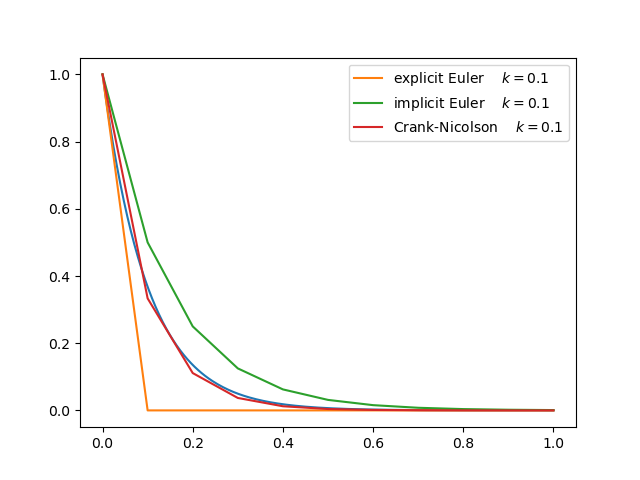
\includegraphics[scale=.4]{4c-ivp-a10-k0-1.png}
      \caption{$a=10, k=0.1$}
  \end{subfigure}
  \begin{subfigure}[b]{.49\linewidth}
      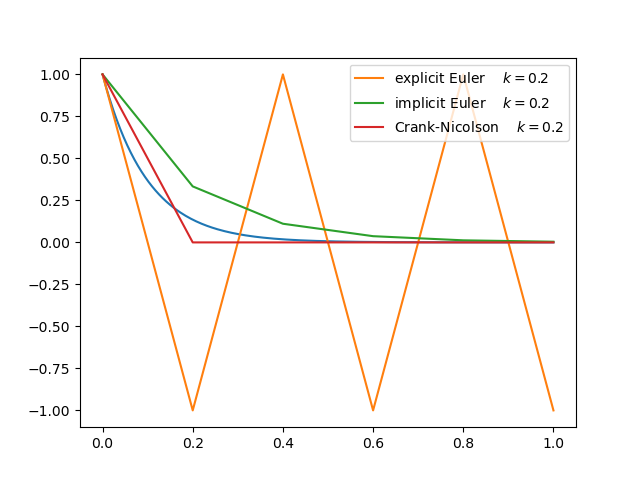
\includegraphics[scale=.4]{4c-ivp-a10-k0-2.png}
      \caption{$a=10, k=0.2$}
  \end{subfigure}
  \hfill
  \begin{subfigure}[b]{.49\linewidth}
      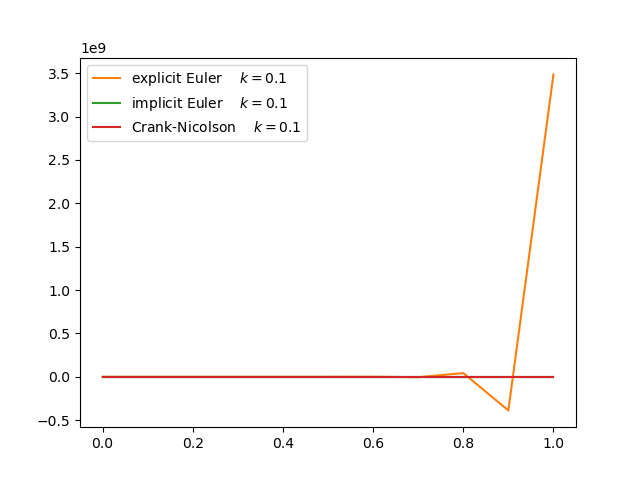
\includegraphics[scale=.4]{4c-ivp-a100-k0-1.png}
      \caption{$a=100, k=0.1$}
  \end{subfigure}
  \begin{subfigure}[b]{.49\linewidth}
      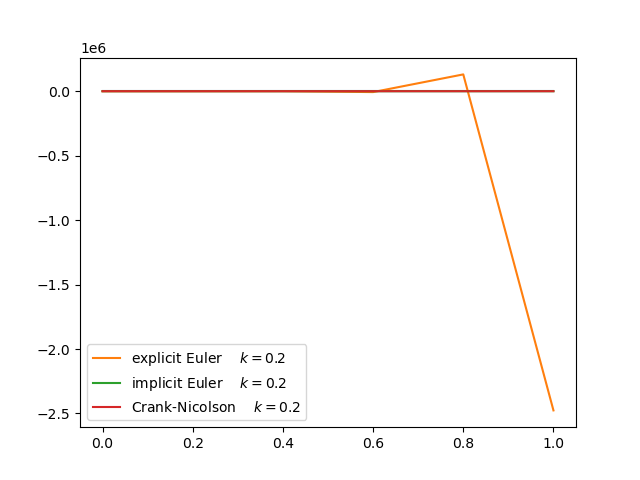
\includegraphics[scale=.4]{4c-ivp-a100-k0-2.png}
      \caption{$a=100, k=0.2$}
  \end{subfigure}

  \caption{Results for the different numerical schemes for the IVP in section~\ref{sec:question4c},
    for different values of $a$ and $k$.
    The exact solution is shown in blue. \label{fig:4c-ivp}}
\end{figure}

\appendix
\section{Source Code}
\lstinputlisting[language=Python]{ass1.py}

\end{document}
